\begin{enumerate}[label=\thesubsection.\arabic*.,ref=\thesubsection.\theenumi]
\numberwithin{equation}{enumi}
\numberwithin{figure}{enumi}
\item $\vec{D}_1$ is a point on $BC$ such that
		\begin{align}
			AD_1 \perp BC
		\end{align}
		and $AD_1$ is defined to be the altitude. 
		Find the normal vector of $AD_1$.
  \\
		
%iffalse
\let\negmedspace\undefined
\let\negthickspace\undefined
\documentclass[journal,12pt,onecolumn]{IEEEtran}
\usepackage[version=4]{mhchem}
\usepackage{chemformula} % for \ch if needed
\usepackage{chemfig}
\usepackage{chemmacros}
\chemsetup{modules = reactions} % Enables reaction arrows

\usepackage{fancyhdr}
\usepackage{geometry}
\usepackage{lastpage}
\usepackage{cite}
\usepackage{amsmath,amssymb,amsfonts,amsthm}
\usepackage{enumitem,multicol}
\usepackage{algorithmic}
\usepackage{graphicx}
\usepackage{textcomp}
\usepackage{xcolor}
\usepackage{txfonts}
\usepackage{listings}
\usepackage{enumitem}
\usepackage{mathtools}
\usepackage{gensymb}
\usepackage{comment}
\usepackage[breaklinks=true]{hyperref}
\usepackage{tkz-euclide} 
\usepackage{listings}
\usepackage{gvv}                                        
%\def\inputGnumericTable{}                                 
\usepackage[utf8]{inputenc}                                
\usepackage{color}                                            
\usepackage{array}                                            
\usepackage{longtable}                                       
\usepackage{calc}                                             
\usepackage{multirow}                                         
\usepackage{hhline}                                           
\usepackage{ifthen}                                           
\usepackage{lscape}
\usepackage{tabularx}
\usepackage{array}
\usepackage{float}

\newtheorem{theorem}{Theorem}[section]
\newtheorem{problem}{Problem}
\newtheorem{proposition}{Proposition}[section]
\newtheorem{lemma}{Lemma}[section]
\newtheorem{corollary}[theorem]{Corollary}
\newtheorem{example}{Example}[section]
\newtheorem{definition}[problem]{Definition}
\newcommand{\BEQA}{\begin{eqnarray}}
\newcommand{\EEQA}{\end{eqnarray}}
\newcommand{\define}{\stackrel{\triangle}{=}}
\theoremstyle{remark}

\geometry{margin=1 in}

% Marks the beginning of the document

\title{\huge {GATE-2010-CE}}
\author{ai25btech11008- Chiruvella Harshith Sharan}
\date{}

\begin{document}

\maketitle

% Reduce spacing between items
\setlength{\parindent}{0pt}
\setlength{\parskip}{0.5cm}

\section*{Q.1 -- Q.25 carry one mark each}

\begin{enumerate}
%------------------- Q1 -------------------%
\item The $\displaystyle \lim_{x \to 0} \frac{\sin \left( \frac{2}{3} x \right)}{x}$ is  
\hfill{\brak{\text{GATE CE 2010}}}
\begin{enumerate}
   
\begin{multicols}{4}
\item  $\dfrac{2}{3}$ 
\item  $1$ 
\item $\dfrac{3}{2}$ 
\item $\infty$
\end{multicols}
\end{enumerate}
%------------------- Q2 -------------------%
\noindent\item Two coins are simultaneously tossed. The probability of two heads simultaneously appearing is \hfill{\brak{\text{GATE CE 2010}}}
\begin{enumerate}
\begin{multicols}{4}
\item $\dfrac{1}{8}$ 
\item $\dfrac{1}{6}$ 
 \item$\dfrac{1}{4}$ 
\item $\dfrac{1}{2}$
\end{multicols}
\end{enumerate}
%------------------- Q3 -------------------%
\noindent\item The order and degree of the differential equation 
\begin{align*}
\frac{d^3 y}{dx^3} + 4 \left( \frac{dy}{dx} \right)^2 + y^2 = 0
\end{align*}
are respectively \hfill{\brak{\text{GATE CE 2010}}}
\begin{enumerate}
\begin{multicols}{4}
\item 3 and 2 
\item2 and 3 
\item 3 and 3 
\item3 and 1
\end{multicols}
\end{enumerate}
%------------------- Q4 -------------------%
\noindent\item Two people weighing $W$ each are sitting on a plank of length $L$ floating on water at $\frac{L}{4}$ from either end. Neglecting the weight of the plank, the bending moment at the centre of the plank is \hfill{\brak{\text{GATE CE 2010}}}
\begin{enumerate}
\begin{multicols}{4}
\item $\dfrac{WL}{8}$ 
\item $\dfrac{WL}{16}$ 
\item $\dfrac{WL}{32}$ 
\item zero
\end{multicols}
\end{enumerate}
%------------------- Q5 -------------------%
\noindent\item For the truss shown in the figure, the force in the member QR is \hfill{\brak{\text{GATE CE 2010}}}
\begin{figure}[H]
    \centering
    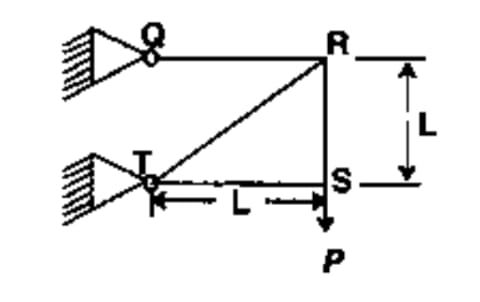
\includegraphics[scale=0.5]{figs/image1.jpg}
    \caption{}
    \label{fig:figure1}
\end{figure}
\begin{enumerate}
\begin{multicols}{4}
\item zero 
\item $\dfrac{P}{\sqrt{2}}$ 
\item $P$ 
\item $\sqrt{2}P$
\end{multicols}
\end{enumerate}
%------------------- Q6 -------------------%
\noindent\item The major and minor principal stresses at a point are 3 MPa and -3 MPa respectively. The maximum shear stress at the point is \hfill{\brak{\text{GATE CE 2010}}}
\begin{enumerate}
\begin{multicols}{4}
\item zero 
\item 3 MPa 
\item 6 MPa 
\item 9 MPa
\end{multicols}
\end{enumerate}
%------------------- Q7 -------------------%
\noindent\item  The number of independent elastic constants for a linear elastic isotropic and homogeneous material is \hfill{\brak{\text{GATE CE 2010}}}
\begin{enumerate}
\begin{multicols}{4}
\item 4 
\item 3 
\item 2 
\item 1
\end{multicols}
\end{enumerate}
%------------------- Q8 -------------------%
\noindent\item The effective length of a column of length $L$ fixed against rotation and translation at one end and free at the other end is \hfill{\brak{\text{GATE CE 2010}}}
\begin{enumerate}
\begin{multicols}{4}
\item $0.5L$ 
\item $0.7L$ 
\item $1.414L$ 
\item $2L$
\end{multicols}
\end{enumerate}

\raggedright
%------------------- Q9 -------------------%
\noindent\item As per Indian standard code of practice for prestressed concrete (IS:1343-1980) the minimum grades of concrete to be used for post-tensioned and pre-tensioned structural elements are respectively 
\hfill{\brak{\text{GATE CE 2010}}}
\begin{enumerate}
\begin{multicols}{4}
\item M20 for both 
\item M40 and M30 
\item M15 and M20 
\item M30 and M40
\end{multicols}
\end{enumerate}
%------------------- Q10 -------------------%
\noindent\item A solid circular shaft of diameter $d$ and length $L$ is fixed at one end and free at the other end. A torque $T$ is applied at the free end. The shear modulus of the material is $G$. The angle of twist at the free end is 
\hfill{\brak{\text{GATE CE 2010}}}
\begin{enumerate}
\begin{multicols}{4}
\item $\dfrac{16TL}{\pi d^4 G}$ 
\item $\dfrac{32TL}{\pi d^4 G}$ 
\item $\dfrac{64TL}{\pi d^4 G}$ 
\item $\dfrac{128TL}{\pi d^4 G}$
\end{multicols}
\end{enumerate}
%------------------- Q11 -------------------%
\noindent\item In a compaction test, $G$, $w$, $S$ and $e$ represent the specific gravity, water content, degree of saturation and void ratio of the soil sample, respectively. If $\gamma_w$ represents the unit weight of water and $\gamma_d$ represents the dry unit weight of the soil, the equation for zero air voids line is 
\\ \hfill{\brak{\text{GATE CE 2010}}}
\begin{enumerate}
\begin{multicols}{4}
\item $\gamma_d = \dfrac{G \gamma_w}{1+Se}$ 
\item $\gamma_d = \dfrac{G \gamma_w}{1+Gw}$ 
\item $\gamma_d = \dfrac{G_w}{e+\gamma_w S}$ 
\item $\gamma_d = \dfrac{G_w}{1+Se}$
\end{multicols}
\end{enumerate}
%------------------- Q12 -------------------%
\noindent\item A fine grained soil has liquid limit of 60 and plastic limit of 20. As per the plasticity chart, according to IS classification, the soil is represented by the letter symbols 
\hfill{\brak{\text{GATE CE 2010}}}
\begin{enumerate}
\begin{multicols}{4}
\item CL 
\item CI 
\item CH 
\item CL-ML
\end{multicols}
\end{enumerate}
%------------------- Q13 -------------------%
\noindent\item Quick sand condition occurs when 
\hfill{\brak{\text{GATE CE 2010}}}


\begin{enumerate}[label=]
 \item A. the void ratio of the soil becomes 1.0 
 \item B. the upward seepage pressure in soil becomes zero 
 \item C. the upward seepage pressure in soil becomes equal to the saturated unit weight of the soil 
 \item D. the upward seepage pressure in soil becomes equal to the submerged unit weight of the soil
 \end{enumerate}


%------------------- Q14 -------------------%
\noindent\item The $e$--$\log p$ curve shown in the figure is representative of 
\hfill{\brak{\text{GATE CE 2010}}}

\begin{figure}[H]
     \centering
     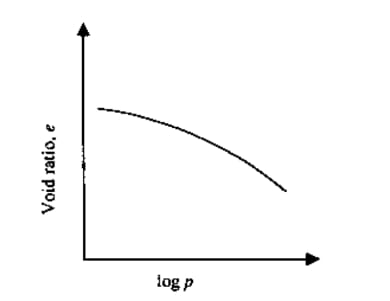
\includegraphics[scale=0.5]{figs/3e0ddfff-16d6-49d4-a917-0f59027d78f5.jpg} 
     \caption{}
     \label{fig:figure2}
 \end{figure}
    
\begin{enumerate}[label=]
\item A. Normally consolidated clay \\
\item B. Over consolidated clay \\
\item C. Under consolidated clay \\
\item D. Normally consolidated clayey sand
\end{enumerate}

% Formatting adjustments
\setlength{\parindent}{0pt}
\setlength{\parskip}{0.5cm}

\raggedright


%------------------- Q15 -------------------%
\noindent\item If $\sigma_h$, $\sigma_v$, $\sigma'_h$ and $\sigma'_v$ represent the total horizontal stress, total vertical stress, effective horizontal stress and effective vertical stress on a soil element, respectively, the coefficient of earth pressure at rest is given by
\hfill{\brak{\text{GATE CE 2010}}}
\begin{enumerate}
\begin{multicols}{4}
\item $\dfrac{\sigma_h}{\sigma_v}$ 
\item $\dfrac{\sigma'_h}{\sigma'_v}$ 
\item $\dfrac{\sigma_v}{\sigma_h}$ 
\item $\dfrac{\sigma'_v}{\sigma'_h}$
\end{multicols}
\end{enumerate}
%------------------- Q16 -------------------%
\noindent\item A mild-sloped channel is followed by a steep-sloped channel. The profiles of gradually varied flow in the channel are
\hfill{\brak{\text{GATE CE 2010}}}
\begin{enumerate}
\begin{multicols}{4}
\item M\textsubscript{1}, S\textsubscript{2} 
\item M\textsubscript{2}, S\textsubscript{3} 
\item M\textsubscript{2}, S\textsubscript{1} 
\item M\textsubscript{2}, S\textsubscript{2}
\end{multicols}
\end{enumerate}
%------------------- Q17 -------------------%
\noindent\item The flow in a rectangular channel is subcritical. If width of the channel is reduced at a certain section, the water surface under no-choke condition will
\hfill{\brak{\text{GATE CE 2010}}}
\begin{enumerate}
\begin{multicols}{4}
\item drop at a downstream section 
\item rise at a downstream section 
\item rise at an upstream section 
\item not undergo any change
\end{multicols}
\end{enumerate}
%------------------- Q18 -------------------%
\noindent\item The correct match of Group-I with Group-II is
\hfill{\brak{\text{GATE CE 2010}}}
\begin{table}[H]
\centering
\begin{tabular}{l l}
Group-I & Group-II \\
P. Evapotranspiration     & 1. Penman method \\
Q. Infiltration    & 2. Snyder’s method \\
R. Synthetic unit hydrograph    & 3. Muskingum method  \\
S. Channel Routing    & 4. Horton's method
\end{tabular}
\label{table1}
\end{table}

\begin{enumerate}
\begin{multicols}{4}
\item P-1, Q-3, R-4, S-2 
\item  P-1, Q-4, R-2, S-3 
\item  P-3, Q-4, R-1, S-2 
\item  P-4, Q-2, R-1, S-3
\end{multicols}
\end{enumerate}
%------------------- Q19 -------------------%
\noindent\item Group-I gives a list of devices and Group-II gives the list of uses. The correct match of Group-I with Group-II is
\hfill{\brak{\text{GATE CE 2010}}}

\begin{table}[H]
    \centering
\begin{tabular}{l l}
Group-I  & Group-II  \\
P. Pitot tube & 1. measuring pressure in a pipe \\
Q. Manometer   & 2. measuring velocity of flow in a pipe     \\
R. Venturimeter     & 3. measuring air and gas velocity          \\
S. Anemometer    & 4. measuring discharge in a pipe
\end{tabular}
\label{table2}
\end{table}

\begin{multicols}{4}
 P-1, Q-2, R-4, S-3 
 P-2, Q-1, R-3, S-4 
 P-2, Q-1, R-4, S-3 
 P-4, Q-1, R-3, S-2
\end{multicols}

%------------------- Q20 -------------------%
\noindent\item A coastal city produces municipal solid waste (MSW) with high moisture content, high organic materials, low calorific value and low inorganic materials. The most effective and sustainable option for MSW management in that city is
\hfill{\brak{\text{GATE CE 2010}}}
\begin{enumerate}
\begin{multicols}{4}
\item Composting 
\item Dumping in sea 
\item Incineration 
\item Landfill
\end{multicols}
\end{enumerate}
%------------------- Q21 -------------------%
\noindent\item According to the Noise Pollution (Regulation and Control) Rules, 2000, of the Ministry of Environment and Forests, India, the day time and night time noise level limits in ambient air for residential areas expressed in dB(A) Leq are
\hfill{\brak{\text{GATE CE 2010}}}
\begin{enumerate}
\begin{multicols}{4}
\item 50 and 40 
\item 55 and 45 
\item 65 and 55 
\item 75 and 70
\end{multicols}
\end{enumerate}
% Formatting adjustments
\setlength{\parindent}{0pt}
\setlength{\parskip}{0.5cm}


%------------------- Q22 -------------------%
\noindent\item An air parcel having $40^\circ\mathrm{C}$ temperature moves from ground level to 500 m elevation in dry air following the ``adiabatic lapse rate''. The resulting temperature of air parcel at 500 m elevation will be
\hfill{\brak{\text{GATE CE 2010}}}
\begin{enumerate}
\begin{multicols}{4}
\item $35^\circ\mathrm{C}$ 
\item $38^\circ\mathrm{C}$ 
\item $41^\circ\mathrm{C}$ 
\item $44^\circ\mathrm{C}$
\end{multicols}
\end{enumerate}
%------------------- Q23 -------------------%
\noindent\item Aggregate impact value indicates the following property of aggregates
\hfill{\brak{\text{GATE CE 2010}}}
\begin{enumerate}
\begin{multicols}{4}
\item Durability 
\item Toughness 
\item Hardness 
\item Strength
\end{multicols}
\end{enumerate}
%------------------- Q24 -------------------%
\noindent\item As per IRC: 67-2001, a traffic sign indicating the Speed Limit on a road should be of               
\hfill{\brak{\text{GATE CE 2010}}}
\begin{enumerate}[label=]
    
\item A.\ Circular Shape with White Background and Red Border \\
\item B.\ Triangular Shape with White Background and Red Border \\
\item C.\ Triangular Shape with Red Background and White Border \\
\item D.\ Circular Shape with Red Background and White Border
\end{enumerate}

%------------------- Q25 -------------------%
\noindent\item The local mean time at a place located in longitude $90^\circ40'$ E when the standard time is 6 hours and 30 minutes and the standard meridian is $82^\circ30'$ E is
\hfill{\brak{\text{GATE CE 2010}}}
\begin{enumerate}[label=]
\item A.\ 5 hours, 2 minutes and 40 seconds \\
\item B.\ 5 hours, 57 minutes and 20 seconds \\
\item C.\ 6 hours and 30 minutes \\
\item D.\ 7 hours, 02 minutes and 40 seconds
\end{enumerate}

\raggedright
    
\section*{Q.26 -- Q.55 carry two marks each}

%------------------- Q26 -----------------%
\noindent\item The solution to the ordinary differential equation
\begin{align*}
\frac{d^2y}{dx^2} + \frac{dy}{dx} - 6y = 0
\end{align*}
is
\hfill{\brak{\text{GATE CE 2010}}}
\begin{enumerate}
\begin{multicols}{4}
\item $y = c_1 e^x + c_2 e^{-2x}$ 
\item $y = c_1 e^{3x} + c_2 e^{2x}$ 
\item $y = c_1 e^{-x} + c_2 e^{-2x}$ 
\item $y = c_1 e^{-3x} + c_2 e^{-2x}$
\end{multicols}
\end{enumerate}
%------------------- Q27 -------------------%
\item The inverse of the matrix \myvec{3+2i & i \\-i & 3-2i} is
\hfill{\brak{\text{GATE CE 2010}}}\newline
\begin{enumerate}
\begin{multicols}{2}
\item $\dfrac{1}{12}$\myvec{ 3+2i & -i \\ i & 3-2j}
\item $\dfrac{1}{12}$\myvec{ 3-2i & -i \\ i & 3+2j}
\item $\dfrac{1}{14}$\myvec{ 3+2i & -i \\ i & 3-2j}
\item $\dfrac{1}{14}$\myvec{ 3-2i & -i \\ i & 3+2j}
\end{multicols}
\end{enumerate}
%------------------- Q28 -------------------%
\noindent\item The table below gives values of a function $F(x)$ obtained for values of $x$ at intervals of 0.25.

\begin{align*}
\begin{array}{c|c|c|c|c|c}
x & 0 & 0.25 & 0.5 & 0.75 & 1.0 \\
\hline
F(x) & 1 & 0.9412 & 0.8 & 0.64 & 0.50
\end{array}
\end{align*}

The value of the integral of the function between the limits 0 to 1 using Simpson's rule is
\\ \hfill{\brak{\text{GATE CE 2010}}}
\begin{enumerate}
\begin{multicols}{4}
\item 0.7854 
\item 2.3562 
\item 3.1416 
\item 7.5000
\end{multicols}
\end{enumerate}

%------------------- Q29 -------------------%
\noindent\item The partial differential equation that can be formed from 
\begin{align*}
z = ax + by + ab
\end{align*}
has the form (with $p = \frac{\partial z}{\partial x}$ and $q = \frac{\partial z}{\partial y}$)
\hfill{\brak{\text{GATE CE 2010}}}
\begin{enumerate}
\begin{multicols}{4}
\item $z = px + qy$ 
\item $z = px + pq$ 
\item $z = px + qy + pq$ 
\item $z = qy + pq$
\end{multicols}
\end{enumerate}
%------------------- Q30 -------------------%
\noindent\item A parabolic cable is held between two supports at the same level. The horizontal span between the supports is $L$. The sag at the mid-span is $h$. The equation of the parabola is 
\begin{align*}
y = \frac{4h}{L^2} x^2
\end{align*}
where $x$ is the horizontal coordinate and $y$ is the vertical coordinate with the origin at the centre of the cable. The expression for the total length of the cable is
\hfill{\brak{\text{GATE CE 2010}}}

A.\ $\int_0^{L/2} \sqrt{1 + 64 \frac{h^2 x^2}{L^4}} \, dx$ \\
B.\ $2 \int_0^{L/2} \sqrt{1 + 64 \frac{h^2 x^2}{L^4}} \, dx$ \\
C.\ $\int_0^{L/2} \sqrt{1 + 64 \frac{h^2 x^2}{L^4}} \, dx$ \\
D.\ $2 \int_0^{L/2} \sqrt{1 + 64 \frac{h^2 x^2}{L^4}} \, dx$

%------------------- Q31 -------------------%
\noindent\item Given a function 
\begin{align*}
f(x, y) = 4x^2 + 6y^2 - 8x - 4y + 8
\end{align*}
The optimal value of $f(x, y)$
\hfill{\brak{\text{GATE CE 2010}}}
\begin{enumerate}
\begin{multicols}{4}
\item is a minimum equal to $10/3$ 
\item is a maximum equal to $10/3$ 
\item is a minimum equal to $8/3$ 
\item is a maximum equal to $8/3$
\end{multicols}
\end{enumerate}
%------------------- Q32 -------------------%
\noindent\item A double cover butt riveted joint is used to connect two flat plates of 200 mm width and 14 mm thickness as shown in the figure. There are twelve power driven rivets of 20 mm diameter at a pitch of 50 mm in both directions on either side of the plate. Two cover plates of 10 mm thickness are used. The capacity of the joint in tension considering bearing and shear ONLY, with permissible bearing and shear stresses as 300 MPa and 100 MPa respectively is
\hfill{\brak{\text{GATE CE 2010}}}

\begin{figure}[H]
     \centering
     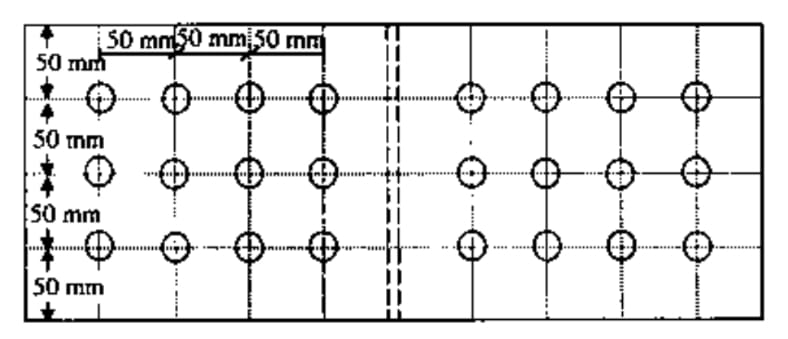
\includegraphics[scale=0.5]{figs/8332fb3c-532c-4d6c-a8c4-1f20c3321f4f.jpg} 
     \caption{}
     \label{fig:figure3}
 \end{figure}
\begin{enumerate}
\begin{multicols}{4}
\item 1083.6 kN 
\item 871.32 kN 
\item 541.8 kN 
\item 433.7 kN
\end{multicols}
\end{enumerate}
%------------------- Q33 -------------------%
\noindent\item Two plates, subjected to direct tension, each of 10 mm thickness and having widths of 100 mm and 175 mm, respectively are to be fillet welded with an overlap of 200 mm. Given that the permissible weld stress is 110 MPa and the permissible stress in steel is 150 MPa, the length of the weld required using the maximum permissible weld size as per IS:800-1984 is \hfill{\brak{\text{GATE CE 2010}}}

\begin{figure}[H]
     \centering
     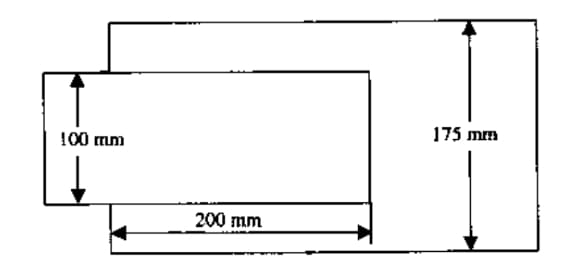
\includegraphics[scale=0.5]{figs/47c2880c-f6f6-44c0-8945-4aa142a40d60.jpg} 
     \caption{}
     \label{fig:figure4}
 \end{figure}
 \begin{enumerate}
\begin{multicols}{4}
\item 245.3 mm 
\item 229.2 mm 
\item 205.5 mm 
\item 194.8 mm
\end{multicols}
\end{enumerate}
%------------------- Q34 -------------------%
\noindent\item For the simply supported beam of length $L$, subjected to a uniformly distributed moment $M$ kN-m per unit length as shown in the figure, the bending moment (in kN-m) at the mid-span of the beam is
\hfill{\brak{\text{GATE CE 2010}}}

\begin{figure}[H]
     \centering
     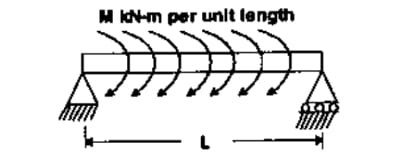
\includegraphics[scale=0.55]{figs/3d041fea-5713-4739-aa3e-a69aaeca9879.jpg} 
     \caption{}
     \label{fig:figure5}
 \end{figure}
 \begin{enumerate}
\begin{multicols}{4}
\item zero 
\item $M$ 
\item $ML$ 
\item $M/L$
\end{multicols}
\end{enumerate}
%------------------- Q35 -------------------%
\noindent\item A disc of radius $r$ has a hole of radius $\frac{r}{2}$ cut-out as shown. The centroid of the remaining disc (shaded portion) at a radial distance from the centre “O” is

\hfill{\brak{\text{GATE CE 2010}}}

\begin{figure}[H]
     \centering
     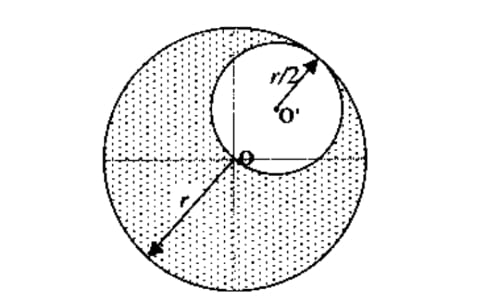
\includegraphics[scale=0.55]{figs/412a18c6-0377-40d3-8e64-77d6fc371075.jpg} 
     \caption{}
     \label{fig:figure6}
 \end{figure}
\begin{enumerate}
\begin{multicols}{4}
\item $\frac{r}{2}$ 
\item $\frac{r}{3}$ 
\item $\frac{r}{6}$ 
\item $\frac{r}{8}$
\end{multicols}
\end{enumerate}

%------------------- Q36 -------------------%
\noindent\item A three hinged parabolic arch having a span of 20 m and a rise of 5 m carries a point load of 10 kN at quarter span from the left end as shown in the figure. The resultant reaction at the left support and its inclination with the horizontal are respectively
\hfill{\brak{\text{GATE CE 2010}}}

\begin{figure}[H]
     \centering
     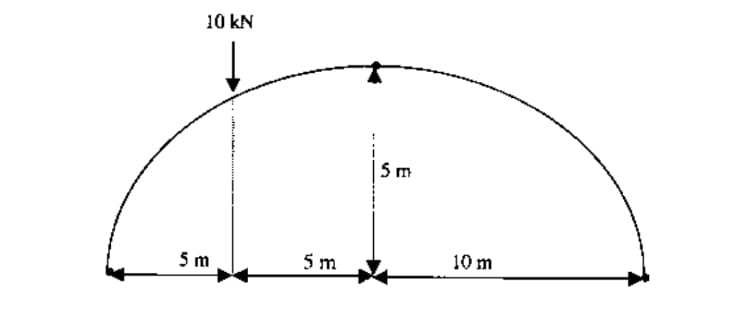
\includegraphics[scale=0.55]{figs/32b8c197-51f7-4381-b234-407edc801822.jpg} 
     \caption{}
     \label{fig:figure7}
 \end{figure}
\begin{enumerate}
\begin{multicols}{2}
\item 9.01 kN and $56.31^\circ$ 
\item 9.01 kN and $33.69^\circ$ 
\item 7.50 kN and $56.31^\circ$ 
\item 2.50 kN and $33.69^\circ$
\end{multicols}
\end{enumerate}
%------------------- Q37 -------------------%
\noindent\item The vertical stress at point $P_1$ due to the point load $Q$ on the ground surface as shown in figure is $\sigma_z$. According to Boussinesq's equation, the vertical stress at point $P_2$ shown in figure will be
\hfill{\brak{\text{GATE CE 2010}}}

\begin{figure}[H]
     \centering
     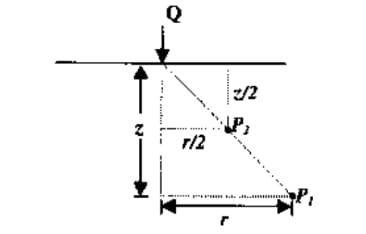
\includegraphics[scale=0.55]{figs/e4388fce-713b-4dc9-a1a5-4b431f7ae7ed.jpg} 
     \caption{}
     \label{fig:figure8}
 \end{figure}
\begin{enumerate}
\begin{multicols}{4}
\item $\frac{\sigma_z}{2}$ 
\item $\sigma_z$ 
\item $2\sigma_z$ 
\item $4\sigma_z$
\end{multicols}
\end{enumerate}
%------------------- Q38 -------------------%
\noindent\item An open ended steel barrel of 1 m height and 1 m diameter is filled with saturated fine sand having coefficient of permeability of $10^{-2}$ m/s. The barrel stands on a saturated bed of gravel. The time required for the water level in the barrel to drop by 0.75 m is \hfill{\brak{\text{GATE CE 2010}}}
\begin{enumerate}
\begin{multicols}{4}
\item 58.9 s 
\item 75 s 
\item 100 s 
\item 150 s
\end{multicols}
\end{enumerate}
%------------------- Q39 -------------------%
\noindent\item The ultimate load capacity of a 10 m long concrete pile of square cross section 500 mm $\times$ 500 mm driven into a homogeneous clay layer having undrained cohesion value of 40 kPa is 700 kN. If the cross section of the pile is reduced to 250 mm $\times$ 250 mm and the length of the pile is increased to 20 m, the ultimate load capacity will be
\hfill{\brak{\text{GATE CE 2010}}}
\begin{enumerate}
\begin{multicols}{4}
\item 350 kN 
\item 632.5 kN 
\item 722.5 kN 
\item 1400 kN
\end{multicols}
\end{enumerate}
\setlength{\parindent}{0pt}
\setlength{\parskip}{0.5cm}


%------------------- Q40 -------------------%
\noindent\item For a rectangular channel section, {Group-I} lists geometrical elements and {Group-II} gives proportions for hydraulically efficient section. 

\begin{table}[H]
\centering
\begin{tabular}{l l}
Group-I & Group-II  \\
P. Top width     & 1. $y_c/2$ \\
Q. Perimeter    & 2.  $y_c$     \\
R. Hydraulic Radius    & 3.  $2y_c$          \\
S. Hydraulic Depth    & 4. $y_c$
\end{tabular}
\label{table3}
\end{table}
$y_c$ is the flow depth corresponding to hydraulically efficient sections. The correct match of {Group-I} with {Group-II} is
\hfill{\brak{\text{GATE CE 2010}}}
\begin{enumerate}
\begin{multicols}{4}
\item P-2, Q-4, R-1, S-3 
\item  P-3, Q-1, R-4, S-2 
\item  P-3, Q-4, R-1, S-2 
\item  P-3, Q-4, R-2, S-1
\end{multicols}
\end{enumerate}
%------------------- Q41 -------------------%
\noindent\item The Froude number of flow in a rectangular channel is 0.8. If the depth of flow is 1.5 m, the critical depth is
\hfill{\brak{\text{GATE CE 2010}}}
\begin{enumerate}
\begin{multicols}{4}
\item 1.80 m 
\item 1.56 m 
\item 1.36 m 
\item 1.29 m
\end{multicols}
\end{enumerate}
%------------------- Q42 -------------------%
\noindent\item A well of diameter 20 cm fully penetrates a confined aquifer. After a long period of pumping at a rate of 2720 litres per minute, the observations of drawdown taken at 10 m and 100 m distances from the center of the well are found to be 3 m and 0.5 m respectively. The transmissivity of the aquifer is
\hfill{\brak{\text{GATE CE 2010}}}
\begin{enumerate}
\begin{multicols}{4}
\item 676 m$^2$/day 
\item 576 m$^2$/day 
\item 526 m$^2$/day 
\item 249 m$^2$/day
\end{multicols}
\end{enumerate}
%------------------- Q43 -------------------%
\noindent\item If the BOD$_5$ of a wastewater sample is 75 mg/L and reaction rate constant $k$ (base $e$) is 0.345 per day, the amount of BOD remaining in the given sample after 10 days is
\hfill{\brak{\text{GATE CE 2010}}}
\begin{enumerate}
\begin{multicols}{4}
\item 3.21 mg/L 
\item 3.45 mg/L 
\item 3.69 mg/L 
\item 3.92 mg/L
\end{multicols}
\end{enumerate}
%------------------- Q44 -------------------%
\noindent\item Consider the following statements in the context of geometric design of roads: \\begin{align*}0.1cm]
I: A simple parabolic curve is an acceptable shape for summit curves \\ 
II: Comfort to passengers is an important consideration in the design of summit curves \\begin{align*}0.2cm]
The correct option evaluating the above statements and their relationship is
\hfill{\brak{\text{GATE CE 2010}}}\newline
A.\ I is true, II is false \\
B.\ I is true, II is true, and II is the correct reason for I \\
C.\ I is true, II is true, and II is NOT the correct reason for I \\
D.\ I is false, II is true

%------------------- Q45 -------------------%
\noindent\item The design speed for a two-lane road is 80 kmph. When a design vehicle with a wheelbase of 6.6 m is negotiating a horizontal curve on that road, the off-tracking is measured as 0.096 m. The required widening of carriageway of the two-lane road on the curve is approximately
\\ \hfill{\brak{\text{GATE CE 2010}}}
\begin{enumerate}
\begin{multicols}{4}
\item 0.55 m 
\item 0.65 m 
\item 0.75 m 
\item 0.85 m
\end{multicols}
\end{enumerate}
%------------------- Q46 -------------------%
\noindent\item Consider the following statements in the context of cement concrete pavements: \\begin{align*}0.1cm]
I: Warping stresses in cement concrete pavements are caused by the seasonal variation in temperature \\ 
II: Tie bars are generally provided across transverse joints of cement concrete pavements \\begin{align*}0.2cm]
The correct option evaluating the above statements is
\hfill{\brak{\text{GATE CE 2010}}}
\begin{enumerate}
\begin{multicols}{4}
\item I: True, II: False 
\item I: False, II: True 
\item I: True, II: True 
\item I: False, II: False
\end{multicols}
\end{enumerate}
%47%
\noindent\item A bench mark has been established at the soffit of an ornamental arch at the known elevation of 100.0 m above mean sea level. The back sight used to establish height of instrument is an inverted staff reading of 2.105 m. A forward sight reading with normally held staff of 1.105 m is taken on a recently constructed plinth. The elevation of the plinth is

\setlength{\parskip}{0.5cm}

\hfill{\brak{\text{GATE CE 2010}}}
\begin{enumerate}
\begin{multicols}{4}
\item 103.210 m
\item 101.000 m
\item 99.000 m
\item 96.790 m
\end{multicols}
\end{enumerate}

\setlength{\parskip}{0.5cm}

\noindent{Common Data for Questions 48 and 49:}

\noindent Ion concentrations obtained for a groundwater sample (having pH = 8.1) are given below
\begin{table}[H]
\resizebox{\textwidth}{!}{%
\begin{tabular}{|c|c|c|c|c|c|c|}
\hline
Ion & Ca\(^{2+}\) & Mg\(^{2+}\) & Na\(^+\) & HCO\(_3^-\) & SO\(_4^{2-}\) & Cl\(^-\) \\
\hline
Ion concentration (mg/L) & 100 & 6 & 15 & 250 & 45 & 39 \\
\hline
Atomic Weight & Ca = 40 & Mg = 24 & Na = 23 & H = 1, C = 12, O = 16 & S = 32, O = 16 & Cl = 35.5 \\
\hline
\end{tabular}%
}
\label{table4}
\end{table}
%48%
\noindent\item Total hardness (mg/L as CaCO\(_3\)) present in the above water sample is

\setlength{\parskip}{0.5cm}

\hfill{\brak{\text{GATE CE 2010}}}
\begin{enumerate}
\begin{multicols}{4}
\item 205
\item 250
\item 275
\item 308
\end{multicols}
\end{enumerate}
\setlength{\parskip}{0.5cm}
%49%
\noindent\item Carbonate hardness (mg/L as CaCO\(_3\)) present in the above water sample is

\setlength{\parskip}{0.5cm}

\hfill{\brak{\text{GATE CE 2010}}}
\begin{enumerate}
\begin{multicols}{4}
\item 205
\item 250
\item 275
\item 289
\end{multicols}
\end{enumerate}

\setlength{\parskip}{0.5cm}

\noindent{Common Data for Questions 50 and 51:}

\noindent The moisture holding capacity of the soil in a 100 hectare farm is 18 cm/m. The field is to be irrigated when 50 percent of the available moisture in the root zone is depleted. The irrigation water is to be supplied by a pump working for 10 hours a day, and water application efficiency is 75 percent. Details of crops planned for cultivation are as follows

\begin{table}[H]
\centering
\begin{tabular}{|c|c|c|}
\hline
Crop & Root zone depth (m) & Peak rate of moisture use (mm/day) \\
\hline
X & 1.0 & 5.0 \\
Y & 0.8 & 4.0 \\
\hline
\end{tabular}
\label{table5}
\end{table}
%50%
\noindent\item The capacity of irrigation system required to irrigate crop 'X' in 36 hectares is

\setlength{\parskip}{0.5cm}

\hfill{\brak{\text{GATE CE 2010}}}
\begin{enumerate}
\begin{multicols}{4}
\item 83 litres/sec
\item 67 litres/sec
\item 57 litres/sec
\item 53 litres/sec
\end{multicols}
\end{enumerate}

\setlength{\parskip}{0.5cm}
%51%
\noindent\item The area of crop 'Y' that can be irrigated when the available capacity of irrigation system is 40 litres/sec is

\setlength{\parskip}{0.5cm}

\hfill{\brak{\text{GATE CE 2010}}}
\begin{enumerate}
\begin{multicols}{4}
\item 40 hectares
\item 36 hectares
\item 30 hectares
\item 27 hectares
\end{multicols}
\end{enumerate}

\noindent{Statement for Linked Answer Questions 52 and 53:}

A doubly reinforced rectangular concrete beam has a width of 300 mm and an effective depth of 500 mm. The beam is reinforced with 2200 mm\(^2\) of steel in tension and 628 mm\(^2\) of steel in compression. The effective cover for compression steel is 50 mm. Assume that both tension and compression steel yield. The grades of concrete and steel used are M20 and Fe250, respectively. The stress block parameters (rounded off to first two decimal places) for concrete shall be as per IS 456:2000.

\setlength{\parskip}{0.5cm}
%52%
\noindent\item The depth of neutral axis is

\setlength{\parskip}{0.5cm}

\hfill{\brak{\text{GATE CE 2010}}}
\begin{enumerate}
\begin{multicols}{4}
\item 205.30 mm
\item 184.56 mm
\item 160.91 mm
\item 145.30 mm
\end{multicols}
\end{enumerate}

\setlength{\parskip}{0.5cm}
%53%
\noindent\item The moment of resistance of the section is

\setlength{\parskip}{0.5cm}

\hfill{\brak{\text{GATE CE 2010}}}
\begin{enumerate}
\begin{multicols}{4}
\item 206.00 kN-m
\item 209.20 kN-m
\item 236.80 kN-m
\item 251.90 kN-m
\end{multicols}
\end{enumerate}

\setlength{\parskip}{0.5cm}

\noindent{Statement for Linked Answer Questions 54 and 55:}

The unconfined compressive strength of a saturated clay sample is 54 kPa.

\setlength{\parskip}{0.5cm}

\noindent\item The value of cohesion for the clay is

\setlength{\parskip}{0.5cm}

\hfill{\brak{\text{GATE CE 2010}}}
\begin{enumerate}
\begin{multicols}{4}
\item zero
\item 13.5 kPa
\item 27 kPa
\item 54 kPa
\end{multicols}
\end{enumerate}

\setlength{\parskip}{0.5cm}
\noindent\item If a square footing of size 4 m x 4 m is resting on the surface of a deposit of the above clay, the ultimate bearing capacity of the footing (as per Terzaghi’s equation) is

\setlength{\parskip}{0.5cm}

\hfill{\brak{\text{GATE CE 2010}}}
\begin{enumerate}
\begin{multicols}{4}
\item 1600 kPa
\item 316 kPa
\item 200 kPa
\item 100 kPa
\end{multicols}
\end{enumerate}

\section*{General Aptitude (GA) Questions}

\noindent{Q.56 -- Q.60 carry one mark each.}

\setlength{\parskip}{0.5cm}
%56%
\noindent \item \textit{Which of the following options is the closest in meaning to the word below:}\\


\hfill{\brak{\text{GATE CE 2010}}}
\begin{enumerate}
\begin{multicols}{4}
\item cyclic
\item indirect
\item confusing
\item crooked
\end{multicols}
\end{enumerate}

\setlength{\parskip}{0.5cm}
%57%
\noindent\item \textit{The question below consists of a pair of related words followed by four pairs of words. Select the pair that best expresses the relation in the original pair.}\\
Unemployed : Worker \hfill{\brak{\text{GATE CE 2010}}}
\begin{enumerate}
\begin{multicols}{2}
\item fallow : land
\item unaware : sleeper
\item wit : jester
\item renovated : house
\end{multicols}
\end{enumerate}

\setlength{\parskip}{0.5cm}
%58%
\noindent\item \textit{Choose the most appropriate word from the options given below to complete the following sentence:}
%59%
\noindent\textit{If we manage to \rule{2cm}{0.15mm} our natural resources, we would leave a better planet for our children.}

\hfill{\brak{\text{GATE CE 2010}}}
\begin{enumerate}
\begin{multicols}{4}
\item uphold
\item restrain
\item cherish
\item conserve
\end{multicols}
\end{enumerate}

\setlength{\parskip}{0.5cm}

\noindent\item \textit{Choose the most appropriate word from the options given below to complete the following sentence:}

\noindent\textit{His rather casual remarks on politics \rule{2cm}{0.15mm} his lack of seriousness about the subject.}

\hfill{\brak{\text{GATE CE 2010}}}
\begin{enumerate}
\begin{multicols}{4}
\item masked
\item belied
\item betrayed
\item suppressed
\end{multicols}
\end{enumerate}

\setlength{\parskip}{0.5cm}
%60%
\noindent\item 25 persons are in a room. 15 of them play hockey, 17 of them play football and 10 of them play both hockey and football. Then the number of persons playing neither hockey nor football is: \hfill{\brak{\text{GATE CE 2010}}}
\begin{enumerate}
\begin{multicols}{4}
\item 2
\item 17
\item 13
\item 3
\end{multicols}
\end{enumerate}

\setlength{\parskip}{0.5cm}

\noindent{Q.61 -- Q.65 carry two marks each.}

\setlength{\parskip}{0.5cm}

 \textit{Modern warfare has changed from large scale clashes of armies to suppression of civilian populations. Chemical agents that do their work silently appear to be suited to such warfare; and regretfully, there exist people in military establishments who think that chemical agents are useful tools for their cause.}

\vspace{0.3cm}
\noindent\item\textit{ Which of the following statements best sums up the meaning of the above passage:}

\hfill{\brak{\text{GATE CE 2010}}}

A.\ Modern warfare has resulted in civil strife. \\
B.\ Chemical agents are useful in modern warfare.\\
C.\ Use of chemical agents in warfare would be undesirable. \\
D.\ People in military establishments like to use chemical agents in war.

\noindent\item If 137 + 276 = 435, how much is 731 + 672?

\hfill{\brak{\text{GATE CE 2010}}}
\begin{enumerate}
\begin{multicols}{4}
\item 534
\item 1403
\item 1623
\item 1513
\end{multicols}
\end{enumerate}

\setlength{\parskip}{0.5cm}

\noindent\item 5 skilled workers can build a wall in 20 days; 8 semi-skilled workers can build a wall in 25 days; 10 unskilled workers can build a wall in 30 days. If a team has 2 skilled, 6 semi-skilled and 5 unskilled workers, how long will it take to build the wall?

\hfill{\brak{\text{GATE CE 2010}}}
\begin{enumerate}
\begin{multicols}{4}
\item 20 days
\item 18 days
\item 16 days
\item 15 days
\end{multicols}
\end{enumerate}

\setlength{\parskip}{0.5cm}

\noindent\item Given digits 2, 2, 3, 3, 3, 4, 4, 4, 4, how many distinct 4-digit numbers greater than 3000 can be formed?

\hfill{\brak{\text{GATE CE 2010}}}
\begin{enumerate}
\begin{multicols}{4}
\item 50
\item 51
\item 52
\item 54
\end{multicols}
\end{enumerate}

\noindent Hari (H), Gita (G), Irfan (I) and Saira (S) are siblings (i.e. brothers and sisters). All were born on 1\textsuperscript{st} January. The age difference between any two successive siblings (that is born one after another) is less than 3 years. Given the following facts:

\begin{itemize}
  \item[i.] Hari’s age + Gita’s age > Irfan’s age + Saira’s age.
  \item[ii.] The age difference between Gita and Saira is 1 year. However, Gita is not the oldest and Saira is not the youngest.
  \item[iii.] There are no twins.
\end{itemize}

\noindent \item  In what order were they born (oldest first)?

\hfill{\brak{\text{GATE CE 2010}}}
\begin{enumerate}
\begin{multicols}{2}
\item HSIG
\item SGHI
\item IGSH
\item IHSG
\end{multicols}
\end{enumerate}

\begin{center}
\section*{END OF QUESTION PAPER}
\end{center}

\end{enumerate}

\end{document}
	\item Find the equation of $AD_1$.
 \\     \input{solutions/1/3/2/Q1.3.2.tex}

	\item Find the equations of the altitudes $BE_1$ and $CF_1$ to the sides $AC$ and $AB$ respectively. 
  \\     
%iffalse
\let\negmedspace\undefined
\let\negthickspace\undefined
\documentclass[journal,12pt,onecolumn]{IEEEtran}
\usepackage[version=4]{mhchem}
\usepackage{chemformula} % for \ch if needed
\usepackage{chemfig}
\usepackage{chemmacros}
\chemsetup{modules = reactions} % Enables reaction arrows

\usepackage{fancyhdr}
\usepackage{geometry}
\usepackage{lastpage}
\usepackage{cite}
\usepackage{amsmath,amssymb,amsfonts,amsthm}
\usepackage{enumitem,multicol}
\usepackage{algorithmic}
\usepackage{graphicx}
\usepackage{textcomp}
\usepackage{xcolor}
\usepackage{txfonts}
\usepackage{listings}
\usepackage{enumitem}
\usepackage{mathtools}
\usepackage{gensymb}
\usepackage{comment}
\usepackage[breaklinks=true]{hyperref}
\usepackage{tkz-euclide} 
\usepackage{listings}
\usepackage{gvv}                                        
%\def\inputGnumericTable{}                                 
\usepackage[utf8]{inputenc}                                
\usepackage{color}                                            
\usepackage{array}                                            
\usepackage{longtable}                                       
\usepackage{calc}                                             
\usepackage{multirow}                                         
\usepackage{hhline}                                           
\usepackage{ifthen}                                           
\usepackage{lscape}
\usepackage{tabularx}
\usepackage{array}
\usepackage{float}

\newtheorem{theorem}{Theorem}[section]
\newtheorem{problem}{Problem}
\newtheorem{proposition}{Proposition}[section]
\newtheorem{lemma}{Lemma}[section]
\newtheorem{corollary}[theorem]{Corollary}
\newtheorem{example}{Example}[section]
\newtheorem{definition}[problem]{Definition}
\newcommand{\BEQA}{\begin{eqnarray}}
\newcommand{\EEQA}{\end{eqnarray}}
\newcommand{\define}{\stackrel{\triangle}{=}}
\theoremstyle{remark}

\geometry{margin=1 in}

% Marks the beginning of the document

\title{\huge {GATE-2010-CE}}
\author{ai25btech11008- Chiruvella Harshith Sharan}
\date{}

\begin{document}

\maketitle

% Reduce spacing between items
\setlength{\parindent}{0pt}
\setlength{\parskip}{0.5cm}

\section*{Q.1 -- Q.25 carry one mark each}

\begin{enumerate}
%------------------- Q1 -------------------%
\item The $\displaystyle \lim_{x \to 0} \frac{\sin \left( \frac{2}{3} x \right)}{x}$ is  
\hfill{\brak{\text{GATE CE 2010}}}
\begin{enumerate}
   
\begin{multicols}{4}
\item  $\dfrac{2}{3}$ 
\item  $1$ 
\item $\dfrac{3}{2}$ 
\item $\infty$
\end{multicols}
\end{enumerate}
%------------------- Q2 -------------------%
\noindent\item Two coins are simultaneously tossed. The probability of two heads simultaneously appearing is \hfill{\brak{\text{GATE CE 2010}}}
\begin{enumerate}
\begin{multicols}{4}
\item $\dfrac{1}{8}$ 
\item $\dfrac{1}{6}$ 
 \item$\dfrac{1}{4}$ 
\item $\dfrac{1}{2}$
\end{multicols}
\end{enumerate}
%------------------- Q3 -------------------%
\noindent\item The order and degree of the differential equation 
\begin{align*}
\frac{d^3 y}{dx^3} + 4 \left( \frac{dy}{dx} \right)^2 + y^2 = 0
\end{align*}
are respectively \hfill{\brak{\text{GATE CE 2010}}}
\begin{enumerate}
\begin{multicols}{4}
\item 3 and 2 
\item2 and 3 
\item 3 and 3 
\item3 and 1
\end{multicols}
\end{enumerate}
%------------------- Q4 -------------------%
\noindent\item Two people weighing $W$ each are sitting on a plank of length $L$ floating on water at $\frac{L}{4}$ from either end. Neglecting the weight of the plank, the bending moment at the centre of the plank is \hfill{\brak{\text{GATE CE 2010}}}
\begin{enumerate}
\begin{multicols}{4}
\item $\dfrac{WL}{8}$ 
\item $\dfrac{WL}{16}$ 
\item $\dfrac{WL}{32}$ 
\item zero
\end{multicols}
\end{enumerate}
%------------------- Q5 -------------------%
\noindent\item For the truss shown in the figure, the force in the member QR is \hfill{\brak{\text{GATE CE 2010}}}
\begin{figure}[H]
    \centering
    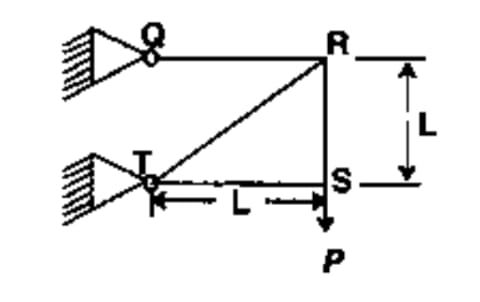
\includegraphics[scale=0.5]{figs/image1.jpg}
    \caption{}
    \label{fig:figure1}
\end{figure}
\begin{enumerate}
\begin{multicols}{4}
\item zero 
\item $\dfrac{P}{\sqrt{2}}$ 
\item $P$ 
\item $\sqrt{2}P$
\end{multicols}
\end{enumerate}
%------------------- Q6 -------------------%
\noindent\item The major and minor principal stresses at a point are 3 MPa and -3 MPa respectively. The maximum shear stress at the point is \hfill{\brak{\text{GATE CE 2010}}}
\begin{enumerate}
\begin{multicols}{4}
\item zero 
\item 3 MPa 
\item 6 MPa 
\item 9 MPa
\end{multicols}
\end{enumerate}
%------------------- Q7 -------------------%
\noindent\item  The number of independent elastic constants for a linear elastic isotropic and homogeneous material is \hfill{\brak{\text{GATE CE 2010}}}
\begin{enumerate}
\begin{multicols}{4}
\item 4 
\item 3 
\item 2 
\item 1
\end{multicols}
\end{enumerate}
%------------------- Q8 -------------------%
\noindent\item The effective length of a column of length $L$ fixed against rotation and translation at one end and free at the other end is \hfill{\brak{\text{GATE CE 2010}}}
\begin{enumerate}
\begin{multicols}{4}
\item $0.5L$ 
\item $0.7L$ 
\item $1.414L$ 
\item $2L$
\end{multicols}
\end{enumerate}

\raggedright
%------------------- Q9 -------------------%
\noindent\item As per Indian standard code of practice for prestressed concrete (IS:1343-1980) the minimum grades of concrete to be used for post-tensioned and pre-tensioned structural elements are respectively 
\hfill{\brak{\text{GATE CE 2010}}}
\begin{enumerate}
\begin{multicols}{4}
\item M20 for both 
\item M40 and M30 
\item M15 and M20 
\item M30 and M40
\end{multicols}
\end{enumerate}
%------------------- Q10 -------------------%
\noindent\item A solid circular shaft of diameter $d$ and length $L$ is fixed at one end and free at the other end. A torque $T$ is applied at the free end. The shear modulus of the material is $G$. The angle of twist at the free end is 
\hfill{\brak{\text{GATE CE 2010}}}
\begin{enumerate}
\begin{multicols}{4}
\item $\dfrac{16TL}{\pi d^4 G}$ 
\item $\dfrac{32TL}{\pi d^4 G}$ 
\item $\dfrac{64TL}{\pi d^4 G}$ 
\item $\dfrac{128TL}{\pi d^4 G}$
\end{multicols}
\end{enumerate}
%------------------- Q11 -------------------%
\noindent\item In a compaction test, $G$, $w$, $S$ and $e$ represent the specific gravity, water content, degree of saturation and void ratio of the soil sample, respectively. If $\gamma_w$ represents the unit weight of water and $\gamma_d$ represents the dry unit weight of the soil, the equation for zero air voids line is 
\\ \hfill{\brak{\text{GATE CE 2010}}}
\begin{enumerate}
\begin{multicols}{4}
\item $\gamma_d = \dfrac{G \gamma_w}{1+Se}$ 
\item $\gamma_d = \dfrac{G \gamma_w}{1+Gw}$ 
\item $\gamma_d = \dfrac{G_w}{e+\gamma_w S}$ 
\item $\gamma_d = \dfrac{G_w}{1+Se}$
\end{multicols}
\end{enumerate}
%------------------- Q12 -------------------%
\noindent\item A fine grained soil has liquid limit of 60 and plastic limit of 20. As per the plasticity chart, according to IS classification, the soil is represented by the letter symbols 
\hfill{\brak{\text{GATE CE 2010}}}
\begin{enumerate}
\begin{multicols}{4}
\item CL 
\item CI 
\item CH 
\item CL-ML
\end{multicols}
\end{enumerate}
%------------------- Q13 -------------------%
\noindent\item Quick sand condition occurs when 
\hfill{\brak{\text{GATE CE 2010}}}


\begin{enumerate}[label=]
 \item A. the void ratio of the soil becomes 1.0 
 \item B. the upward seepage pressure in soil becomes zero 
 \item C. the upward seepage pressure in soil becomes equal to the saturated unit weight of the soil 
 \item D. the upward seepage pressure in soil becomes equal to the submerged unit weight of the soil
 \end{enumerate}


%------------------- Q14 -------------------%
\noindent\item The $e$--$\log p$ curve shown in the figure is representative of 
\hfill{\brak{\text{GATE CE 2010}}}

\begin{figure}[H]
     \centering
     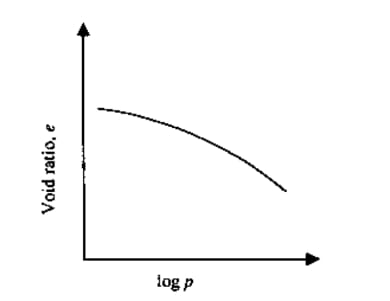
\includegraphics[scale=0.5]{figs/3e0ddfff-16d6-49d4-a917-0f59027d78f5.jpg} 
     \caption{}
     \label{fig:figure2}
 \end{figure}
    
\begin{enumerate}[label=]
\item A. Normally consolidated clay \\
\item B. Over consolidated clay \\
\item C. Under consolidated clay \\
\item D. Normally consolidated clayey sand
\end{enumerate}

% Formatting adjustments
\setlength{\parindent}{0pt}
\setlength{\parskip}{0.5cm}

\raggedright


%------------------- Q15 -------------------%
\noindent\item If $\sigma_h$, $\sigma_v$, $\sigma'_h$ and $\sigma'_v$ represent the total horizontal stress, total vertical stress, effective horizontal stress and effective vertical stress on a soil element, respectively, the coefficient of earth pressure at rest is given by
\hfill{\brak{\text{GATE CE 2010}}}
\begin{enumerate}
\begin{multicols}{4}
\item $\dfrac{\sigma_h}{\sigma_v}$ 
\item $\dfrac{\sigma'_h}{\sigma'_v}$ 
\item $\dfrac{\sigma_v}{\sigma_h}$ 
\item $\dfrac{\sigma'_v}{\sigma'_h}$
\end{multicols}
\end{enumerate}
%------------------- Q16 -------------------%
\noindent\item A mild-sloped channel is followed by a steep-sloped channel. The profiles of gradually varied flow in the channel are
\hfill{\brak{\text{GATE CE 2010}}}
\begin{enumerate}
\begin{multicols}{4}
\item M\textsubscript{1}, S\textsubscript{2} 
\item M\textsubscript{2}, S\textsubscript{3} 
\item M\textsubscript{2}, S\textsubscript{1} 
\item M\textsubscript{2}, S\textsubscript{2}
\end{multicols}
\end{enumerate}
%------------------- Q17 -------------------%
\noindent\item The flow in a rectangular channel is subcritical. If width of the channel is reduced at a certain section, the water surface under no-choke condition will
\hfill{\brak{\text{GATE CE 2010}}}
\begin{enumerate}
\begin{multicols}{4}
\item drop at a downstream section 
\item rise at a downstream section 
\item rise at an upstream section 
\item not undergo any change
\end{multicols}
\end{enumerate}
%------------------- Q18 -------------------%
\noindent\item The correct match of Group-I with Group-II is
\hfill{\brak{\text{GATE CE 2010}}}
\begin{table}[H]
\centering
\begin{tabular}{l l}
Group-I & Group-II \\
P. Evapotranspiration     & 1. Penman method \\
Q. Infiltration    & 2. Snyder’s method \\
R. Synthetic unit hydrograph    & 3. Muskingum method  \\
S. Channel Routing    & 4. Horton's method
\end{tabular}
\label{table1}
\end{table}

\begin{enumerate}
\begin{multicols}{4}
\item P-1, Q-3, R-4, S-2 
\item  P-1, Q-4, R-2, S-3 
\item  P-3, Q-4, R-1, S-2 
\item  P-4, Q-2, R-1, S-3
\end{multicols}
\end{enumerate}
%------------------- Q19 -------------------%
\noindent\item Group-I gives a list of devices and Group-II gives the list of uses. The correct match of Group-I with Group-II is
\hfill{\brak{\text{GATE CE 2010}}}

\begin{table}[H]
    \centering
\begin{tabular}{l l}
Group-I  & Group-II  \\
P. Pitot tube & 1. measuring pressure in a pipe \\
Q. Manometer   & 2. measuring velocity of flow in a pipe     \\
R. Venturimeter     & 3. measuring air and gas velocity          \\
S. Anemometer    & 4. measuring discharge in a pipe
\end{tabular}
\label{table2}
\end{table}

\begin{multicols}{4}
 P-1, Q-2, R-4, S-3 
 P-2, Q-1, R-3, S-4 
 P-2, Q-1, R-4, S-3 
 P-4, Q-1, R-3, S-2
\end{multicols}

%------------------- Q20 -------------------%
\noindent\item A coastal city produces municipal solid waste (MSW) with high moisture content, high organic materials, low calorific value and low inorganic materials. The most effective and sustainable option for MSW management in that city is
\hfill{\brak{\text{GATE CE 2010}}}
\begin{enumerate}
\begin{multicols}{4}
\item Composting 
\item Dumping in sea 
\item Incineration 
\item Landfill
\end{multicols}
\end{enumerate}
%------------------- Q21 -------------------%
\noindent\item According to the Noise Pollution (Regulation and Control) Rules, 2000, of the Ministry of Environment and Forests, India, the day time and night time noise level limits in ambient air for residential areas expressed in dB(A) Leq are
\hfill{\brak{\text{GATE CE 2010}}}
\begin{enumerate}
\begin{multicols}{4}
\item 50 and 40 
\item 55 and 45 
\item 65 and 55 
\item 75 and 70
\end{multicols}
\end{enumerate}
% Formatting adjustments
\setlength{\parindent}{0pt}
\setlength{\parskip}{0.5cm}


%------------------- Q22 -------------------%
\noindent\item An air parcel having $40^\circ\mathrm{C}$ temperature moves from ground level to 500 m elevation in dry air following the ``adiabatic lapse rate''. The resulting temperature of air parcel at 500 m elevation will be
\hfill{\brak{\text{GATE CE 2010}}}
\begin{enumerate}
\begin{multicols}{4}
\item $35^\circ\mathrm{C}$ 
\item $38^\circ\mathrm{C}$ 
\item $41^\circ\mathrm{C}$ 
\item $44^\circ\mathrm{C}$
\end{multicols}
\end{enumerate}
%------------------- Q23 -------------------%
\noindent\item Aggregate impact value indicates the following property of aggregates
\hfill{\brak{\text{GATE CE 2010}}}
\begin{enumerate}
\begin{multicols}{4}
\item Durability 
\item Toughness 
\item Hardness 
\item Strength
\end{multicols}
\end{enumerate}
%------------------- Q24 -------------------%
\noindent\item As per IRC: 67-2001, a traffic sign indicating the Speed Limit on a road should be of               
\hfill{\brak{\text{GATE CE 2010}}}
\begin{enumerate}[label=]
    
\item A.\ Circular Shape with White Background and Red Border \\
\item B.\ Triangular Shape with White Background and Red Border \\
\item C.\ Triangular Shape with Red Background and White Border \\
\item D.\ Circular Shape with Red Background and White Border
\end{enumerate}

%------------------- Q25 -------------------%
\noindent\item The local mean time at a place located in longitude $90^\circ40'$ E when the standard time is 6 hours and 30 minutes and the standard meridian is $82^\circ30'$ E is
\hfill{\brak{\text{GATE CE 2010}}}
\begin{enumerate}[label=]
\item A.\ 5 hours, 2 minutes and 40 seconds \\
\item B.\ 5 hours, 57 minutes and 20 seconds \\
\item C.\ 6 hours and 30 minutes \\
\item D.\ 7 hours, 02 minutes and 40 seconds
\end{enumerate}

\raggedright
    
\section*{Q.26 -- Q.55 carry two marks each}

%------------------- Q26 -----------------%
\noindent\item The solution to the ordinary differential equation
\begin{align*}
\frac{d^2y}{dx^2} + \frac{dy}{dx} - 6y = 0
\end{align*}
is
\hfill{\brak{\text{GATE CE 2010}}}
\begin{enumerate}
\begin{multicols}{4}
\item $y = c_1 e^x + c_2 e^{-2x}$ 
\item $y = c_1 e^{3x} + c_2 e^{2x}$ 
\item $y = c_1 e^{-x} + c_2 e^{-2x}$ 
\item $y = c_1 e^{-3x} + c_2 e^{-2x}$
\end{multicols}
\end{enumerate}
%------------------- Q27 -------------------%
\item The inverse of the matrix \myvec{3+2i & i \\-i & 3-2i} is
\hfill{\brak{\text{GATE CE 2010}}}\newline
\begin{enumerate}
\begin{multicols}{2}
\item $\dfrac{1}{12}$\myvec{ 3+2i & -i \\ i & 3-2j}
\item $\dfrac{1}{12}$\myvec{ 3-2i & -i \\ i & 3+2j}
\item $\dfrac{1}{14}$\myvec{ 3+2i & -i \\ i & 3-2j}
\item $\dfrac{1}{14}$\myvec{ 3-2i & -i \\ i & 3+2j}
\end{multicols}
\end{enumerate}
%------------------- Q28 -------------------%
\noindent\item The table below gives values of a function $F(x)$ obtained for values of $x$ at intervals of 0.25.

\begin{align*}
\begin{array}{c|c|c|c|c|c}
x & 0 & 0.25 & 0.5 & 0.75 & 1.0 \\
\hline
F(x) & 1 & 0.9412 & 0.8 & 0.64 & 0.50
\end{array}
\end{align*}

The value of the integral of the function between the limits 0 to 1 using Simpson's rule is
\\ \hfill{\brak{\text{GATE CE 2010}}}
\begin{enumerate}
\begin{multicols}{4}
\item 0.7854 
\item 2.3562 
\item 3.1416 
\item 7.5000
\end{multicols}
\end{enumerate}

%------------------- Q29 -------------------%
\noindent\item The partial differential equation that can be formed from 
\begin{align*}
z = ax + by + ab
\end{align*}
has the form (with $p = \frac{\partial z}{\partial x}$ and $q = \frac{\partial z}{\partial y}$)
\hfill{\brak{\text{GATE CE 2010}}}
\begin{enumerate}
\begin{multicols}{4}
\item $z = px + qy$ 
\item $z = px + pq$ 
\item $z = px + qy + pq$ 
\item $z = qy + pq$
\end{multicols}
\end{enumerate}
%------------------- Q30 -------------------%
\noindent\item A parabolic cable is held between two supports at the same level. The horizontal span between the supports is $L$. The sag at the mid-span is $h$. The equation of the parabola is 
\begin{align*}
y = \frac{4h}{L^2} x^2
\end{align*}
where $x$ is the horizontal coordinate and $y$ is the vertical coordinate with the origin at the centre of the cable. The expression for the total length of the cable is
\hfill{\brak{\text{GATE CE 2010}}}

A.\ $\int_0^{L/2} \sqrt{1 + 64 \frac{h^2 x^2}{L^4}} \, dx$ \\
B.\ $2 \int_0^{L/2} \sqrt{1 + 64 \frac{h^2 x^2}{L^4}} \, dx$ \\
C.\ $\int_0^{L/2} \sqrt{1 + 64 \frac{h^2 x^2}{L^4}} \, dx$ \\
D.\ $2 \int_0^{L/2} \sqrt{1 + 64 \frac{h^2 x^2}{L^4}} \, dx$

%------------------- Q31 -------------------%
\noindent\item Given a function 
\begin{align*}
f(x, y) = 4x^2 + 6y^2 - 8x - 4y + 8
\end{align*}
The optimal value of $f(x, y)$
\hfill{\brak{\text{GATE CE 2010}}}
\begin{enumerate}
\begin{multicols}{4}
\item is a minimum equal to $10/3$ 
\item is a maximum equal to $10/3$ 
\item is a minimum equal to $8/3$ 
\item is a maximum equal to $8/3$
\end{multicols}
\end{enumerate}
%------------------- Q32 -------------------%
\noindent\item A double cover butt riveted joint is used to connect two flat plates of 200 mm width and 14 mm thickness as shown in the figure. There are twelve power driven rivets of 20 mm diameter at a pitch of 50 mm in both directions on either side of the plate. Two cover plates of 10 mm thickness are used. The capacity of the joint in tension considering bearing and shear ONLY, with permissible bearing and shear stresses as 300 MPa and 100 MPa respectively is
\hfill{\brak{\text{GATE CE 2010}}}

\begin{figure}[H]
     \centering
     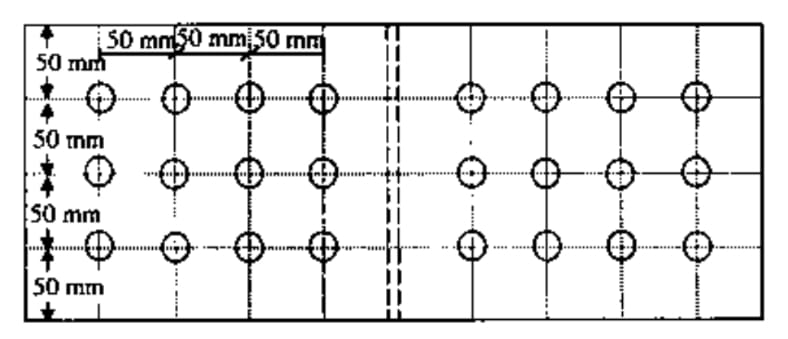
\includegraphics[scale=0.5]{figs/8332fb3c-532c-4d6c-a8c4-1f20c3321f4f.jpg} 
     \caption{}
     \label{fig:figure3}
 \end{figure}
\begin{enumerate}
\begin{multicols}{4}
\item 1083.6 kN 
\item 871.32 kN 
\item 541.8 kN 
\item 433.7 kN
\end{multicols}
\end{enumerate}
%------------------- Q33 -------------------%
\noindent\item Two plates, subjected to direct tension, each of 10 mm thickness and having widths of 100 mm and 175 mm, respectively are to be fillet welded with an overlap of 200 mm. Given that the permissible weld stress is 110 MPa and the permissible stress in steel is 150 MPa, the length of the weld required using the maximum permissible weld size as per IS:800-1984 is \hfill{\brak{\text{GATE CE 2010}}}

\begin{figure}[H]
     \centering
     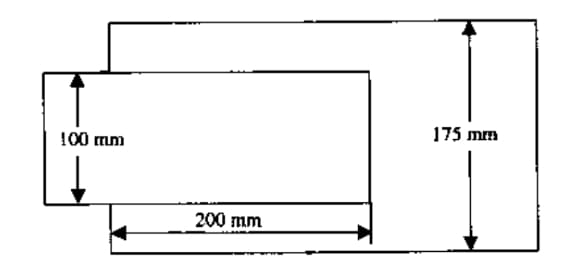
\includegraphics[scale=0.5]{figs/47c2880c-f6f6-44c0-8945-4aa142a40d60.jpg} 
     \caption{}
     \label{fig:figure4}
 \end{figure}
 \begin{enumerate}
\begin{multicols}{4}
\item 245.3 mm 
\item 229.2 mm 
\item 205.5 mm 
\item 194.8 mm
\end{multicols}
\end{enumerate}
%------------------- Q34 -------------------%
\noindent\item For the simply supported beam of length $L$, subjected to a uniformly distributed moment $M$ kN-m per unit length as shown in the figure, the bending moment (in kN-m) at the mid-span of the beam is
\hfill{\brak{\text{GATE CE 2010}}}

\begin{figure}[H]
     \centering
     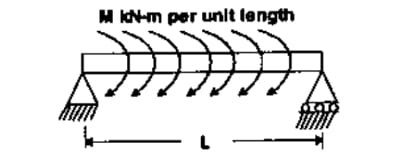
\includegraphics[scale=0.55]{figs/3d041fea-5713-4739-aa3e-a69aaeca9879.jpg} 
     \caption{}
     \label{fig:figure5}
 \end{figure}
 \begin{enumerate}
\begin{multicols}{4}
\item zero 
\item $M$ 
\item $ML$ 
\item $M/L$
\end{multicols}
\end{enumerate}
%------------------- Q35 -------------------%
\noindent\item A disc of radius $r$ has a hole of radius $\frac{r}{2}$ cut-out as shown. The centroid of the remaining disc (shaded portion) at a radial distance from the centre “O” is

\hfill{\brak{\text{GATE CE 2010}}}

\begin{figure}[H]
     \centering
     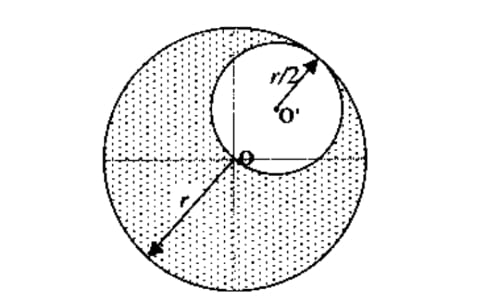
\includegraphics[scale=0.55]{figs/412a18c6-0377-40d3-8e64-77d6fc371075.jpg} 
     \caption{}
     \label{fig:figure6}
 \end{figure}
\begin{enumerate}
\begin{multicols}{4}
\item $\frac{r}{2}$ 
\item $\frac{r}{3}$ 
\item $\frac{r}{6}$ 
\item $\frac{r}{8}$
\end{multicols}
\end{enumerate}

%------------------- Q36 -------------------%
\noindent\item A three hinged parabolic arch having a span of 20 m and a rise of 5 m carries a point load of 10 kN at quarter span from the left end as shown in the figure. The resultant reaction at the left support and its inclination with the horizontal are respectively
\hfill{\brak{\text{GATE CE 2010}}}

\begin{figure}[H]
     \centering
     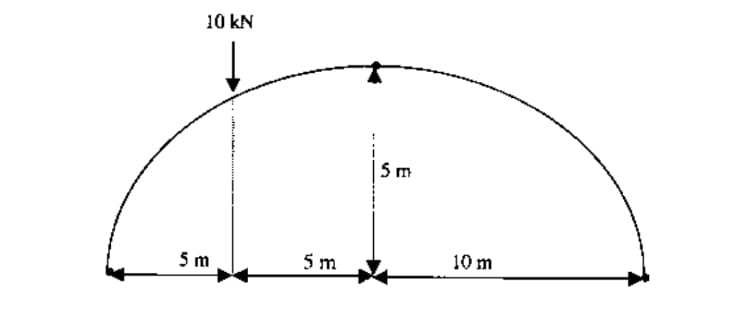
\includegraphics[scale=0.55]{figs/32b8c197-51f7-4381-b234-407edc801822.jpg} 
     \caption{}
     \label{fig:figure7}
 \end{figure}
\begin{enumerate}
\begin{multicols}{2}
\item 9.01 kN and $56.31^\circ$ 
\item 9.01 kN and $33.69^\circ$ 
\item 7.50 kN and $56.31^\circ$ 
\item 2.50 kN and $33.69^\circ$
\end{multicols}
\end{enumerate}
%------------------- Q37 -------------------%
\noindent\item The vertical stress at point $P_1$ due to the point load $Q$ on the ground surface as shown in figure is $\sigma_z$. According to Boussinesq's equation, the vertical stress at point $P_2$ shown in figure will be
\hfill{\brak{\text{GATE CE 2010}}}

\begin{figure}[H]
     \centering
     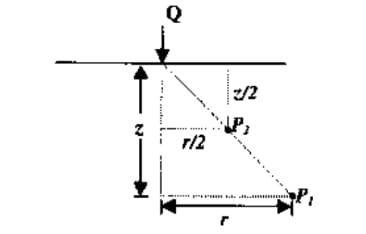
\includegraphics[scale=0.55]{figs/e4388fce-713b-4dc9-a1a5-4b431f7ae7ed.jpg} 
     \caption{}
     \label{fig:figure8}
 \end{figure}
\begin{enumerate}
\begin{multicols}{4}
\item $\frac{\sigma_z}{2}$ 
\item $\sigma_z$ 
\item $2\sigma_z$ 
\item $4\sigma_z$
\end{multicols}
\end{enumerate}
%------------------- Q38 -------------------%
\noindent\item An open ended steel barrel of 1 m height and 1 m diameter is filled with saturated fine sand having coefficient of permeability of $10^{-2}$ m/s. The barrel stands on a saturated bed of gravel. The time required for the water level in the barrel to drop by 0.75 m is \hfill{\brak{\text{GATE CE 2010}}}
\begin{enumerate}
\begin{multicols}{4}
\item 58.9 s 
\item 75 s 
\item 100 s 
\item 150 s
\end{multicols}
\end{enumerate}
%------------------- Q39 -------------------%
\noindent\item The ultimate load capacity of a 10 m long concrete pile of square cross section 500 mm $\times$ 500 mm driven into a homogeneous clay layer having undrained cohesion value of 40 kPa is 700 kN. If the cross section of the pile is reduced to 250 mm $\times$ 250 mm and the length of the pile is increased to 20 m, the ultimate load capacity will be
\hfill{\brak{\text{GATE CE 2010}}}
\begin{enumerate}
\begin{multicols}{4}
\item 350 kN 
\item 632.5 kN 
\item 722.5 kN 
\item 1400 kN
\end{multicols}
\end{enumerate}
\setlength{\parindent}{0pt}
\setlength{\parskip}{0.5cm}


%------------------- Q40 -------------------%
\noindent\item For a rectangular channel section, {Group-I} lists geometrical elements and {Group-II} gives proportions for hydraulically efficient section. 

\begin{table}[H]
\centering
\begin{tabular}{l l}
Group-I & Group-II  \\
P. Top width     & 1. $y_c/2$ \\
Q. Perimeter    & 2.  $y_c$     \\
R. Hydraulic Radius    & 3.  $2y_c$          \\
S. Hydraulic Depth    & 4. $y_c$
\end{tabular}
\label{table3}
\end{table}
$y_c$ is the flow depth corresponding to hydraulically efficient sections. The correct match of {Group-I} with {Group-II} is
\hfill{\brak{\text{GATE CE 2010}}}
\begin{enumerate}
\begin{multicols}{4}
\item P-2, Q-4, R-1, S-3 
\item  P-3, Q-1, R-4, S-2 
\item  P-3, Q-4, R-1, S-2 
\item  P-3, Q-4, R-2, S-1
\end{multicols}
\end{enumerate}
%------------------- Q41 -------------------%
\noindent\item The Froude number of flow in a rectangular channel is 0.8. If the depth of flow is 1.5 m, the critical depth is
\hfill{\brak{\text{GATE CE 2010}}}
\begin{enumerate}
\begin{multicols}{4}
\item 1.80 m 
\item 1.56 m 
\item 1.36 m 
\item 1.29 m
\end{multicols}
\end{enumerate}
%------------------- Q42 -------------------%
\noindent\item A well of diameter 20 cm fully penetrates a confined aquifer. After a long period of pumping at a rate of 2720 litres per minute, the observations of drawdown taken at 10 m and 100 m distances from the center of the well are found to be 3 m and 0.5 m respectively. The transmissivity of the aquifer is
\hfill{\brak{\text{GATE CE 2010}}}
\begin{enumerate}
\begin{multicols}{4}
\item 676 m$^2$/day 
\item 576 m$^2$/day 
\item 526 m$^2$/day 
\item 249 m$^2$/day
\end{multicols}
\end{enumerate}
%------------------- Q43 -------------------%
\noindent\item If the BOD$_5$ of a wastewater sample is 75 mg/L and reaction rate constant $k$ (base $e$) is 0.345 per day, the amount of BOD remaining in the given sample after 10 days is
\hfill{\brak{\text{GATE CE 2010}}}
\begin{enumerate}
\begin{multicols}{4}
\item 3.21 mg/L 
\item 3.45 mg/L 
\item 3.69 mg/L 
\item 3.92 mg/L
\end{multicols}
\end{enumerate}
%------------------- Q44 -------------------%
\noindent\item Consider the following statements in the context of geometric design of roads: \\begin{align*}0.1cm]
I: A simple parabolic curve is an acceptable shape for summit curves \\ 
II: Comfort to passengers is an important consideration in the design of summit curves \\begin{align*}0.2cm]
The correct option evaluating the above statements and their relationship is
\hfill{\brak{\text{GATE CE 2010}}}\newline
A.\ I is true, II is false \\
B.\ I is true, II is true, and II is the correct reason for I \\
C.\ I is true, II is true, and II is NOT the correct reason for I \\
D.\ I is false, II is true

%------------------- Q45 -------------------%
\noindent\item The design speed for a two-lane road is 80 kmph. When a design vehicle with a wheelbase of 6.6 m is negotiating a horizontal curve on that road, the off-tracking is measured as 0.096 m. The required widening of carriageway of the two-lane road on the curve is approximately
\\ \hfill{\brak{\text{GATE CE 2010}}}
\begin{enumerate}
\begin{multicols}{4}
\item 0.55 m 
\item 0.65 m 
\item 0.75 m 
\item 0.85 m
\end{multicols}
\end{enumerate}
%------------------- Q46 -------------------%
\noindent\item Consider the following statements in the context of cement concrete pavements: \\begin{align*}0.1cm]
I: Warping stresses in cement concrete pavements are caused by the seasonal variation in temperature \\ 
II: Tie bars are generally provided across transverse joints of cement concrete pavements \\begin{align*}0.2cm]
The correct option evaluating the above statements is
\hfill{\brak{\text{GATE CE 2010}}}
\begin{enumerate}
\begin{multicols}{4}
\item I: True, II: False 
\item I: False, II: True 
\item I: True, II: True 
\item I: False, II: False
\end{multicols}
\end{enumerate}
%47%
\noindent\item A bench mark has been established at the soffit of an ornamental arch at the known elevation of 100.0 m above mean sea level. The back sight used to establish height of instrument is an inverted staff reading of 2.105 m. A forward sight reading with normally held staff of 1.105 m is taken on a recently constructed plinth. The elevation of the plinth is

\setlength{\parskip}{0.5cm}

\hfill{\brak{\text{GATE CE 2010}}}
\begin{enumerate}
\begin{multicols}{4}
\item 103.210 m
\item 101.000 m
\item 99.000 m
\item 96.790 m
\end{multicols}
\end{enumerate}

\setlength{\parskip}{0.5cm}

\noindent{Common Data for Questions 48 and 49:}

\noindent Ion concentrations obtained for a groundwater sample (having pH = 8.1) are given below
\begin{table}[H]
\resizebox{\textwidth}{!}{%
\begin{tabular}{|c|c|c|c|c|c|c|}
\hline
Ion & Ca\(^{2+}\) & Mg\(^{2+}\) & Na\(^+\) & HCO\(_3^-\) & SO\(_4^{2-}\) & Cl\(^-\) \\
\hline
Ion concentration (mg/L) & 100 & 6 & 15 & 250 & 45 & 39 \\
\hline
Atomic Weight & Ca = 40 & Mg = 24 & Na = 23 & H = 1, C = 12, O = 16 & S = 32, O = 16 & Cl = 35.5 \\
\hline
\end{tabular}%
}
\label{table4}
\end{table}
%48%
\noindent\item Total hardness (mg/L as CaCO\(_3\)) present in the above water sample is

\setlength{\parskip}{0.5cm}

\hfill{\brak{\text{GATE CE 2010}}}
\begin{enumerate}
\begin{multicols}{4}
\item 205
\item 250
\item 275
\item 308
\end{multicols}
\end{enumerate}
\setlength{\parskip}{0.5cm}
%49%
\noindent\item Carbonate hardness (mg/L as CaCO\(_3\)) present in the above water sample is

\setlength{\parskip}{0.5cm}

\hfill{\brak{\text{GATE CE 2010}}}
\begin{enumerate}
\begin{multicols}{4}
\item 205
\item 250
\item 275
\item 289
\end{multicols}
\end{enumerate}

\setlength{\parskip}{0.5cm}

\noindent{Common Data for Questions 50 and 51:}

\noindent The moisture holding capacity of the soil in a 100 hectare farm is 18 cm/m. The field is to be irrigated when 50 percent of the available moisture in the root zone is depleted. The irrigation water is to be supplied by a pump working for 10 hours a day, and water application efficiency is 75 percent. Details of crops planned for cultivation are as follows

\begin{table}[H]
\centering
\begin{tabular}{|c|c|c|}
\hline
Crop & Root zone depth (m) & Peak rate of moisture use (mm/day) \\
\hline
X & 1.0 & 5.0 \\
Y & 0.8 & 4.0 \\
\hline
\end{tabular}
\label{table5}
\end{table}
%50%
\noindent\item The capacity of irrigation system required to irrigate crop 'X' in 36 hectares is

\setlength{\parskip}{0.5cm}

\hfill{\brak{\text{GATE CE 2010}}}
\begin{enumerate}
\begin{multicols}{4}
\item 83 litres/sec
\item 67 litres/sec
\item 57 litres/sec
\item 53 litres/sec
\end{multicols}
\end{enumerate}

\setlength{\parskip}{0.5cm}
%51%
\noindent\item The area of crop 'Y' that can be irrigated when the available capacity of irrigation system is 40 litres/sec is

\setlength{\parskip}{0.5cm}

\hfill{\brak{\text{GATE CE 2010}}}
\begin{enumerate}
\begin{multicols}{4}
\item 40 hectares
\item 36 hectares
\item 30 hectares
\item 27 hectares
\end{multicols}
\end{enumerate}

\noindent{Statement for Linked Answer Questions 52 and 53:}

A doubly reinforced rectangular concrete beam has a width of 300 mm and an effective depth of 500 mm. The beam is reinforced with 2200 mm\(^2\) of steel in tension and 628 mm\(^2\) of steel in compression. The effective cover for compression steel is 50 mm. Assume that both tension and compression steel yield. The grades of concrete and steel used are M20 and Fe250, respectively. The stress block parameters (rounded off to first two decimal places) for concrete shall be as per IS 456:2000.

\setlength{\parskip}{0.5cm}
%52%
\noindent\item The depth of neutral axis is

\setlength{\parskip}{0.5cm}

\hfill{\brak{\text{GATE CE 2010}}}
\begin{enumerate}
\begin{multicols}{4}
\item 205.30 mm
\item 184.56 mm
\item 160.91 mm
\item 145.30 mm
\end{multicols}
\end{enumerate}

\setlength{\parskip}{0.5cm}
%53%
\noindent\item The moment of resistance of the section is

\setlength{\parskip}{0.5cm}

\hfill{\brak{\text{GATE CE 2010}}}
\begin{enumerate}
\begin{multicols}{4}
\item 206.00 kN-m
\item 209.20 kN-m
\item 236.80 kN-m
\item 251.90 kN-m
\end{multicols}
\end{enumerate}

\setlength{\parskip}{0.5cm}

\noindent{Statement for Linked Answer Questions 54 and 55:}

The unconfined compressive strength of a saturated clay sample is 54 kPa.

\setlength{\parskip}{0.5cm}

\noindent\item The value of cohesion for the clay is

\setlength{\parskip}{0.5cm}

\hfill{\brak{\text{GATE CE 2010}}}
\begin{enumerate}
\begin{multicols}{4}
\item zero
\item 13.5 kPa
\item 27 kPa
\item 54 kPa
\end{multicols}
\end{enumerate}

\setlength{\parskip}{0.5cm}
\noindent\item If a square footing of size 4 m x 4 m is resting on the surface of a deposit of the above clay, the ultimate bearing capacity of the footing (as per Terzaghi’s equation) is

\setlength{\parskip}{0.5cm}

\hfill{\brak{\text{GATE CE 2010}}}
\begin{enumerate}
\begin{multicols}{4}
\item 1600 kPa
\item 316 kPa
\item 200 kPa
\item 100 kPa
\end{multicols}
\end{enumerate}

\section*{General Aptitude (GA) Questions}

\noindent{Q.56 -- Q.60 carry one mark each.}

\setlength{\parskip}{0.5cm}
%56%
\noindent \item \textit{Which of the following options is the closest in meaning to the word below:}\\


\hfill{\brak{\text{GATE CE 2010}}}
\begin{enumerate}
\begin{multicols}{4}
\item cyclic
\item indirect
\item confusing
\item crooked
\end{multicols}
\end{enumerate}

\setlength{\parskip}{0.5cm}
%57%
\noindent\item \textit{The question below consists of a pair of related words followed by four pairs of words. Select the pair that best expresses the relation in the original pair.}\\
Unemployed : Worker \hfill{\brak{\text{GATE CE 2010}}}
\begin{enumerate}
\begin{multicols}{2}
\item fallow : land
\item unaware : sleeper
\item wit : jester
\item renovated : house
\end{multicols}
\end{enumerate}

\setlength{\parskip}{0.5cm}
%58%
\noindent\item \textit{Choose the most appropriate word from the options given below to complete the following sentence:}
%59%
\noindent\textit{If we manage to \rule{2cm}{0.15mm} our natural resources, we would leave a better planet for our children.}

\hfill{\brak{\text{GATE CE 2010}}}
\begin{enumerate}
\begin{multicols}{4}
\item uphold
\item restrain
\item cherish
\item conserve
\end{multicols}
\end{enumerate}

\setlength{\parskip}{0.5cm}

\noindent\item \textit{Choose the most appropriate word from the options given below to complete the following sentence:}

\noindent\textit{His rather casual remarks on politics \rule{2cm}{0.15mm} his lack of seriousness about the subject.}

\hfill{\brak{\text{GATE CE 2010}}}
\begin{enumerate}
\begin{multicols}{4}
\item masked
\item belied
\item betrayed
\item suppressed
\end{multicols}
\end{enumerate}

\setlength{\parskip}{0.5cm}
%60%
\noindent\item 25 persons are in a room. 15 of them play hockey, 17 of them play football and 10 of them play both hockey and football. Then the number of persons playing neither hockey nor football is: \hfill{\brak{\text{GATE CE 2010}}}
\begin{enumerate}
\begin{multicols}{4}
\item 2
\item 17
\item 13
\item 3
\end{multicols}
\end{enumerate}

\setlength{\parskip}{0.5cm}

\noindent{Q.61 -- Q.65 carry two marks each.}

\setlength{\parskip}{0.5cm}

 \textit{Modern warfare has changed from large scale clashes of armies to suppression of civilian populations. Chemical agents that do their work silently appear to be suited to such warfare; and regretfully, there exist people in military establishments who think that chemical agents are useful tools for their cause.}

\vspace{0.3cm}
\noindent\item\textit{ Which of the following statements best sums up the meaning of the above passage:}

\hfill{\brak{\text{GATE CE 2010}}}

A.\ Modern warfare has resulted in civil strife. \\
B.\ Chemical agents are useful in modern warfare.\\
C.\ Use of chemical agents in warfare would be undesirable. \\
D.\ People in military establishments like to use chemical agents in war.

\noindent\item If 137 + 276 = 435, how much is 731 + 672?

\hfill{\brak{\text{GATE CE 2010}}}
\begin{enumerate}
\begin{multicols}{4}
\item 534
\item 1403
\item 1623
\item 1513
\end{multicols}
\end{enumerate}

\setlength{\parskip}{0.5cm}

\noindent\item 5 skilled workers can build a wall in 20 days; 8 semi-skilled workers can build a wall in 25 days; 10 unskilled workers can build a wall in 30 days. If a team has 2 skilled, 6 semi-skilled and 5 unskilled workers, how long will it take to build the wall?

\hfill{\brak{\text{GATE CE 2010}}}
\begin{enumerate}
\begin{multicols}{4}
\item 20 days
\item 18 days
\item 16 days
\item 15 days
\end{multicols}
\end{enumerate}

\setlength{\parskip}{0.5cm}

\noindent\item Given digits 2, 2, 3, 3, 3, 4, 4, 4, 4, how many distinct 4-digit numbers greater than 3000 can be formed?

\hfill{\brak{\text{GATE CE 2010}}}
\begin{enumerate}
\begin{multicols}{4}
\item 50
\item 51
\item 52
\item 54
\end{multicols}
\end{enumerate}

\noindent Hari (H), Gita (G), Irfan (I) and Saira (S) are siblings (i.e. brothers and sisters). All were born on 1\textsuperscript{st} January. The age difference between any two successive siblings (that is born one after another) is less than 3 years. Given the following facts:

\begin{itemize}
  \item[i.] Hari’s age + Gita’s age > Irfan’s age + Saira’s age.
  \item[ii.] The age difference between Gita and Saira is 1 year. However, Gita is not the oldest and Saira is not the youngest.
  \item[iii.] There are no twins.
\end{itemize}

\noindent \item  In what order were they born (oldest first)?

\hfill{\brak{\text{GATE CE 2010}}}
\begin{enumerate}
\begin{multicols}{2}
\item HSIG
\item SGHI
\item IGSH
\item IHSG
\end{multicols}
\end{enumerate}

\begin{center}
\section*{END OF QUESTION PAPER}
\end{center}

\end{enumerate}

\end{document}
	\item Find the intersection $\vec{H}$ of $BE_1$ and $CF_1$.
 \\
        
%iffalse
\let\negmedspace\undefined
\let\negthickspace\undefined
\documentclass[journal,12pt,onecolumn]{IEEEtran}
\usepackage[version=4]{mhchem}
\usepackage{chemformula} % for \ch if needed
\usepackage{chemfig}
\usepackage{chemmacros}
\chemsetup{modules = reactions} % Enables reaction arrows

\usepackage{fancyhdr}
\usepackage{geometry}
\usepackage{lastpage}
\usepackage{cite}
\usepackage{amsmath,amssymb,amsfonts,amsthm}
\usepackage{enumitem,multicol}
\usepackage{algorithmic}
\usepackage{graphicx}
\usepackage{textcomp}
\usepackage{xcolor}
\usepackage{txfonts}
\usepackage{listings}
\usepackage{enumitem}
\usepackage{mathtools}
\usepackage{gensymb}
\usepackage{comment}
\usepackage[breaklinks=true]{hyperref}
\usepackage{tkz-euclide} 
\usepackage{listings}
\usepackage{gvv}                                        
%\def\inputGnumericTable{}                                 
\usepackage[utf8]{inputenc}                                
\usepackage{color}                                            
\usepackage{array}                                            
\usepackage{longtable}                                       
\usepackage{calc}                                             
\usepackage{multirow}                                         
\usepackage{hhline}                                           
\usepackage{ifthen}                                           
\usepackage{lscape}
\usepackage{tabularx}
\usepackage{array}
\usepackage{float}

\newtheorem{theorem}{Theorem}[section]
\newtheorem{problem}{Problem}
\newtheorem{proposition}{Proposition}[section]
\newtheorem{lemma}{Lemma}[section]
\newtheorem{corollary}[theorem]{Corollary}
\newtheorem{example}{Example}[section]
\newtheorem{definition}[problem]{Definition}
\newcommand{\BEQA}{\begin{eqnarray}}
\newcommand{\EEQA}{\end{eqnarray}}
\newcommand{\define}{\stackrel{\triangle}{=}}
\theoremstyle{remark}

\geometry{margin=1 in}

% Marks the beginning of the document

\title{\huge {GATE-2010-CE}}
\author{ai25btech11008- Chiruvella Harshith Sharan}
\date{}

\begin{document}

\maketitle

% Reduce spacing between items
\setlength{\parindent}{0pt}
\setlength{\parskip}{0.5cm}

\section*{Q.1 -- Q.25 carry one mark each}

\begin{enumerate}
%------------------- Q1 -------------------%
\item The $\displaystyle \lim_{x \to 0} \frac{\sin \left( \frac{2}{3} x \right)}{x}$ is  
\hfill{\brak{\text{GATE CE 2010}}}
\begin{enumerate}
   
\begin{multicols}{4}
\item  $\dfrac{2}{3}$ 
\item  $1$ 
\item $\dfrac{3}{2}$ 
\item $\infty$
\end{multicols}
\end{enumerate}
%------------------- Q2 -------------------%
\noindent\item Two coins are simultaneously tossed. The probability of two heads simultaneously appearing is \hfill{\brak{\text{GATE CE 2010}}}
\begin{enumerate}
\begin{multicols}{4}
\item $\dfrac{1}{8}$ 
\item $\dfrac{1}{6}$ 
 \item$\dfrac{1}{4}$ 
\item $\dfrac{1}{2}$
\end{multicols}
\end{enumerate}
%------------------- Q3 -------------------%
\noindent\item The order and degree of the differential equation 
\begin{align*}
\frac{d^3 y}{dx^3} + 4 \left( \frac{dy}{dx} \right)^2 + y^2 = 0
\end{align*}
are respectively \hfill{\brak{\text{GATE CE 2010}}}
\begin{enumerate}
\begin{multicols}{4}
\item 3 and 2 
\item2 and 3 
\item 3 and 3 
\item3 and 1
\end{multicols}
\end{enumerate}
%------------------- Q4 -------------------%
\noindent\item Two people weighing $W$ each are sitting on a plank of length $L$ floating on water at $\frac{L}{4}$ from either end. Neglecting the weight of the plank, the bending moment at the centre of the plank is \hfill{\brak{\text{GATE CE 2010}}}
\begin{enumerate}
\begin{multicols}{4}
\item $\dfrac{WL}{8}$ 
\item $\dfrac{WL}{16}$ 
\item $\dfrac{WL}{32}$ 
\item zero
\end{multicols}
\end{enumerate}
%------------------- Q5 -------------------%
\noindent\item For the truss shown in the figure, the force in the member QR is \hfill{\brak{\text{GATE CE 2010}}}
\begin{figure}[H]
    \centering
    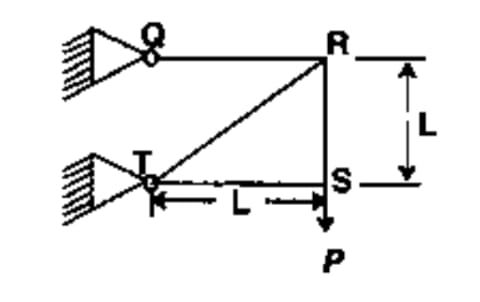
\includegraphics[scale=0.5]{figs/image1.jpg}
    \caption{}
    \label{fig:figure1}
\end{figure}
\begin{enumerate}
\begin{multicols}{4}
\item zero 
\item $\dfrac{P}{\sqrt{2}}$ 
\item $P$ 
\item $\sqrt{2}P$
\end{multicols}
\end{enumerate}
%------------------- Q6 -------------------%
\noindent\item The major and minor principal stresses at a point are 3 MPa and -3 MPa respectively. The maximum shear stress at the point is \hfill{\brak{\text{GATE CE 2010}}}
\begin{enumerate}
\begin{multicols}{4}
\item zero 
\item 3 MPa 
\item 6 MPa 
\item 9 MPa
\end{multicols}
\end{enumerate}
%------------------- Q7 -------------------%
\noindent\item  The number of independent elastic constants for a linear elastic isotropic and homogeneous material is \hfill{\brak{\text{GATE CE 2010}}}
\begin{enumerate}
\begin{multicols}{4}
\item 4 
\item 3 
\item 2 
\item 1
\end{multicols}
\end{enumerate}
%------------------- Q8 -------------------%
\noindent\item The effective length of a column of length $L$ fixed against rotation and translation at one end and free at the other end is \hfill{\brak{\text{GATE CE 2010}}}
\begin{enumerate}
\begin{multicols}{4}
\item $0.5L$ 
\item $0.7L$ 
\item $1.414L$ 
\item $2L$
\end{multicols}
\end{enumerate}

\raggedright
%------------------- Q9 -------------------%
\noindent\item As per Indian standard code of practice for prestressed concrete (IS:1343-1980) the minimum grades of concrete to be used for post-tensioned and pre-tensioned structural elements are respectively 
\hfill{\brak{\text{GATE CE 2010}}}
\begin{enumerate}
\begin{multicols}{4}
\item M20 for both 
\item M40 and M30 
\item M15 and M20 
\item M30 and M40
\end{multicols}
\end{enumerate}
%------------------- Q10 -------------------%
\noindent\item A solid circular shaft of diameter $d$ and length $L$ is fixed at one end and free at the other end. A torque $T$ is applied at the free end. The shear modulus of the material is $G$. The angle of twist at the free end is 
\hfill{\brak{\text{GATE CE 2010}}}
\begin{enumerate}
\begin{multicols}{4}
\item $\dfrac{16TL}{\pi d^4 G}$ 
\item $\dfrac{32TL}{\pi d^4 G}$ 
\item $\dfrac{64TL}{\pi d^4 G}$ 
\item $\dfrac{128TL}{\pi d^4 G}$
\end{multicols}
\end{enumerate}
%------------------- Q11 -------------------%
\noindent\item In a compaction test, $G$, $w$, $S$ and $e$ represent the specific gravity, water content, degree of saturation and void ratio of the soil sample, respectively. If $\gamma_w$ represents the unit weight of water and $\gamma_d$ represents the dry unit weight of the soil, the equation for zero air voids line is 
\\ \hfill{\brak{\text{GATE CE 2010}}}
\begin{enumerate}
\begin{multicols}{4}
\item $\gamma_d = \dfrac{G \gamma_w}{1+Se}$ 
\item $\gamma_d = \dfrac{G \gamma_w}{1+Gw}$ 
\item $\gamma_d = \dfrac{G_w}{e+\gamma_w S}$ 
\item $\gamma_d = \dfrac{G_w}{1+Se}$
\end{multicols}
\end{enumerate}
%------------------- Q12 -------------------%
\noindent\item A fine grained soil has liquid limit of 60 and plastic limit of 20. As per the plasticity chart, according to IS classification, the soil is represented by the letter symbols 
\hfill{\brak{\text{GATE CE 2010}}}
\begin{enumerate}
\begin{multicols}{4}
\item CL 
\item CI 
\item CH 
\item CL-ML
\end{multicols}
\end{enumerate}
%------------------- Q13 -------------------%
\noindent\item Quick sand condition occurs when 
\hfill{\brak{\text{GATE CE 2010}}}


\begin{enumerate}[label=]
 \item A. the void ratio of the soil becomes 1.0 
 \item B. the upward seepage pressure in soil becomes zero 
 \item C. the upward seepage pressure in soil becomes equal to the saturated unit weight of the soil 
 \item D. the upward seepage pressure in soil becomes equal to the submerged unit weight of the soil
 \end{enumerate}


%------------------- Q14 -------------------%
\noindent\item The $e$--$\log p$ curve shown in the figure is representative of 
\hfill{\brak{\text{GATE CE 2010}}}

\begin{figure}[H]
     \centering
     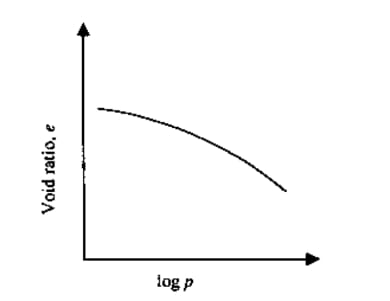
\includegraphics[scale=0.5]{figs/3e0ddfff-16d6-49d4-a917-0f59027d78f5.jpg} 
     \caption{}
     \label{fig:figure2}
 \end{figure}
    
\begin{enumerate}[label=]
\item A. Normally consolidated clay \\
\item B. Over consolidated clay \\
\item C. Under consolidated clay \\
\item D. Normally consolidated clayey sand
\end{enumerate}

% Formatting adjustments
\setlength{\parindent}{0pt}
\setlength{\parskip}{0.5cm}

\raggedright


%------------------- Q15 -------------------%
\noindent\item If $\sigma_h$, $\sigma_v$, $\sigma'_h$ and $\sigma'_v$ represent the total horizontal stress, total vertical stress, effective horizontal stress and effective vertical stress on a soil element, respectively, the coefficient of earth pressure at rest is given by
\hfill{\brak{\text{GATE CE 2010}}}
\begin{enumerate}
\begin{multicols}{4}
\item $\dfrac{\sigma_h}{\sigma_v}$ 
\item $\dfrac{\sigma'_h}{\sigma'_v}$ 
\item $\dfrac{\sigma_v}{\sigma_h}$ 
\item $\dfrac{\sigma'_v}{\sigma'_h}$
\end{multicols}
\end{enumerate}
%------------------- Q16 -------------------%
\noindent\item A mild-sloped channel is followed by a steep-sloped channel. The profiles of gradually varied flow in the channel are
\hfill{\brak{\text{GATE CE 2010}}}
\begin{enumerate}
\begin{multicols}{4}
\item M\textsubscript{1}, S\textsubscript{2} 
\item M\textsubscript{2}, S\textsubscript{3} 
\item M\textsubscript{2}, S\textsubscript{1} 
\item M\textsubscript{2}, S\textsubscript{2}
\end{multicols}
\end{enumerate}
%------------------- Q17 -------------------%
\noindent\item The flow in a rectangular channel is subcritical. If width of the channel is reduced at a certain section, the water surface under no-choke condition will
\hfill{\brak{\text{GATE CE 2010}}}
\begin{enumerate}
\begin{multicols}{4}
\item drop at a downstream section 
\item rise at a downstream section 
\item rise at an upstream section 
\item not undergo any change
\end{multicols}
\end{enumerate}
%------------------- Q18 -------------------%
\noindent\item The correct match of Group-I with Group-II is
\hfill{\brak{\text{GATE CE 2010}}}
\begin{table}[H]
\centering
\begin{tabular}{l l}
Group-I & Group-II \\
P. Evapotranspiration     & 1. Penman method \\
Q. Infiltration    & 2. Snyder’s method \\
R. Synthetic unit hydrograph    & 3. Muskingum method  \\
S. Channel Routing    & 4. Horton's method
\end{tabular}
\label{table1}
\end{table}

\begin{enumerate}
\begin{multicols}{4}
\item P-1, Q-3, R-4, S-2 
\item  P-1, Q-4, R-2, S-3 
\item  P-3, Q-4, R-1, S-2 
\item  P-4, Q-2, R-1, S-3
\end{multicols}
\end{enumerate}
%------------------- Q19 -------------------%
\noindent\item Group-I gives a list of devices and Group-II gives the list of uses. The correct match of Group-I with Group-II is
\hfill{\brak{\text{GATE CE 2010}}}

\begin{table}[H]
    \centering
\begin{tabular}{l l}
Group-I  & Group-II  \\
P. Pitot tube & 1. measuring pressure in a pipe \\
Q. Manometer   & 2. measuring velocity of flow in a pipe     \\
R. Venturimeter     & 3. measuring air and gas velocity          \\
S. Anemometer    & 4. measuring discharge in a pipe
\end{tabular}
\label{table2}
\end{table}

\begin{multicols}{4}
 P-1, Q-2, R-4, S-3 
 P-2, Q-1, R-3, S-4 
 P-2, Q-1, R-4, S-3 
 P-4, Q-1, R-3, S-2
\end{multicols}

%------------------- Q20 -------------------%
\noindent\item A coastal city produces municipal solid waste (MSW) with high moisture content, high organic materials, low calorific value and low inorganic materials. The most effective and sustainable option for MSW management in that city is
\hfill{\brak{\text{GATE CE 2010}}}
\begin{enumerate}
\begin{multicols}{4}
\item Composting 
\item Dumping in sea 
\item Incineration 
\item Landfill
\end{multicols}
\end{enumerate}
%------------------- Q21 -------------------%
\noindent\item According to the Noise Pollution (Regulation and Control) Rules, 2000, of the Ministry of Environment and Forests, India, the day time and night time noise level limits in ambient air for residential areas expressed in dB(A) Leq are
\hfill{\brak{\text{GATE CE 2010}}}
\begin{enumerate}
\begin{multicols}{4}
\item 50 and 40 
\item 55 and 45 
\item 65 and 55 
\item 75 and 70
\end{multicols}
\end{enumerate}
% Formatting adjustments
\setlength{\parindent}{0pt}
\setlength{\parskip}{0.5cm}


%------------------- Q22 -------------------%
\noindent\item An air parcel having $40^\circ\mathrm{C}$ temperature moves from ground level to 500 m elevation in dry air following the ``adiabatic lapse rate''. The resulting temperature of air parcel at 500 m elevation will be
\hfill{\brak{\text{GATE CE 2010}}}
\begin{enumerate}
\begin{multicols}{4}
\item $35^\circ\mathrm{C}$ 
\item $38^\circ\mathrm{C}$ 
\item $41^\circ\mathrm{C}$ 
\item $44^\circ\mathrm{C}$
\end{multicols}
\end{enumerate}
%------------------- Q23 -------------------%
\noindent\item Aggregate impact value indicates the following property of aggregates
\hfill{\brak{\text{GATE CE 2010}}}
\begin{enumerate}
\begin{multicols}{4}
\item Durability 
\item Toughness 
\item Hardness 
\item Strength
\end{multicols}
\end{enumerate}
%------------------- Q24 -------------------%
\noindent\item As per IRC: 67-2001, a traffic sign indicating the Speed Limit on a road should be of               
\hfill{\brak{\text{GATE CE 2010}}}
\begin{enumerate}[label=]
    
\item A.\ Circular Shape with White Background and Red Border \\
\item B.\ Triangular Shape with White Background and Red Border \\
\item C.\ Triangular Shape with Red Background and White Border \\
\item D.\ Circular Shape with Red Background and White Border
\end{enumerate}

%------------------- Q25 -------------------%
\noindent\item The local mean time at a place located in longitude $90^\circ40'$ E when the standard time is 6 hours and 30 minutes and the standard meridian is $82^\circ30'$ E is
\hfill{\brak{\text{GATE CE 2010}}}
\begin{enumerate}[label=]
\item A.\ 5 hours, 2 minutes and 40 seconds \\
\item B.\ 5 hours, 57 minutes and 20 seconds \\
\item C.\ 6 hours and 30 minutes \\
\item D.\ 7 hours, 02 minutes and 40 seconds
\end{enumerate}

\raggedright
    
\section*{Q.26 -- Q.55 carry two marks each}

%------------------- Q26 -----------------%
\noindent\item The solution to the ordinary differential equation
\begin{align*}
\frac{d^2y}{dx^2} + \frac{dy}{dx} - 6y = 0
\end{align*}
is
\hfill{\brak{\text{GATE CE 2010}}}
\begin{enumerate}
\begin{multicols}{4}
\item $y = c_1 e^x + c_2 e^{-2x}$ 
\item $y = c_1 e^{3x} + c_2 e^{2x}$ 
\item $y = c_1 e^{-x} + c_2 e^{-2x}$ 
\item $y = c_1 e^{-3x} + c_2 e^{-2x}$
\end{multicols}
\end{enumerate}
%------------------- Q27 -------------------%
\item The inverse of the matrix \myvec{3+2i & i \\-i & 3-2i} is
\hfill{\brak{\text{GATE CE 2010}}}\newline
\begin{enumerate}
\begin{multicols}{2}
\item $\dfrac{1}{12}$\myvec{ 3+2i & -i \\ i & 3-2j}
\item $\dfrac{1}{12}$\myvec{ 3-2i & -i \\ i & 3+2j}
\item $\dfrac{1}{14}$\myvec{ 3+2i & -i \\ i & 3-2j}
\item $\dfrac{1}{14}$\myvec{ 3-2i & -i \\ i & 3+2j}
\end{multicols}
\end{enumerate}
%------------------- Q28 -------------------%
\noindent\item The table below gives values of a function $F(x)$ obtained for values of $x$ at intervals of 0.25.

\begin{align*}
\begin{array}{c|c|c|c|c|c}
x & 0 & 0.25 & 0.5 & 0.75 & 1.0 \\
\hline
F(x) & 1 & 0.9412 & 0.8 & 0.64 & 0.50
\end{array}
\end{align*}

The value of the integral of the function between the limits 0 to 1 using Simpson's rule is
\\ \hfill{\brak{\text{GATE CE 2010}}}
\begin{enumerate}
\begin{multicols}{4}
\item 0.7854 
\item 2.3562 
\item 3.1416 
\item 7.5000
\end{multicols}
\end{enumerate}

%------------------- Q29 -------------------%
\noindent\item The partial differential equation that can be formed from 
\begin{align*}
z = ax + by + ab
\end{align*}
has the form (with $p = \frac{\partial z}{\partial x}$ and $q = \frac{\partial z}{\partial y}$)
\hfill{\brak{\text{GATE CE 2010}}}
\begin{enumerate}
\begin{multicols}{4}
\item $z = px + qy$ 
\item $z = px + pq$ 
\item $z = px + qy + pq$ 
\item $z = qy + pq$
\end{multicols}
\end{enumerate}
%------------------- Q30 -------------------%
\noindent\item A parabolic cable is held between two supports at the same level. The horizontal span between the supports is $L$. The sag at the mid-span is $h$. The equation of the parabola is 
\begin{align*}
y = \frac{4h}{L^2} x^2
\end{align*}
where $x$ is the horizontal coordinate and $y$ is the vertical coordinate with the origin at the centre of the cable. The expression for the total length of the cable is
\hfill{\brak{\text{GATE CE 2010}}}

A.\ $\int_0^{L/2} \sqrt{1 + 64 \frac{h^2 x^2}{L^4}} \, dx$ \\
B.\ $2 \int_0^{L/2} \sqrt{1 + 64 \frac{h^2 x^2}{L^4}} \, dx$ \\
C.\ $\int_0^{L/2} \sqrt{1 + 64 \frac{h^2 x^2}{L^4}} \, dx$ \\
D.\ $2 \int_0^{L/2} \sqrt{1 + 64 \frac{h^2 x^2}{L^4}} \, dx$

%------------------- Q31 -------------------%
\noindent\item Given a function 
\begin{align*}
f(x, y) = 4x^2 + 6y^2 - 8x - 4y + 8
\end{align*}
The optimal value of $f(x, y)$
\hfill{\brak{\text{GATE CE 2010}}}
\begin{enumerate}
\begin{multicols}{4}
\item is a minimum equal to $10/3$ 
\item is a maximum equal to $10/3$ 
\item is a minimum equal to $8/3$ 
\item is a maximum equal to $8/3$
\end{multicols}
\end{enumerate}
%------------------- Q32 -------------------%
\noindent\item A double cover butt riveted joint is used to connect two flat plates of 200 mm width and 14 mm thickness as shown in the figure. There are twelve power driven rivets of 20 mm diameter at a pitch of 50 mm in both directions on either side of the plate. Two cover plates of 10 mm thickness are used. The capacity of the joint in tension considering bearing and shear ONLY, with permissible bearing and shear stresses as 300 MPa and 100 MPa respectively is
\hfill{\brak{\text{GATE CE 2010}}}

\begin{figure}[H]
     \centering
     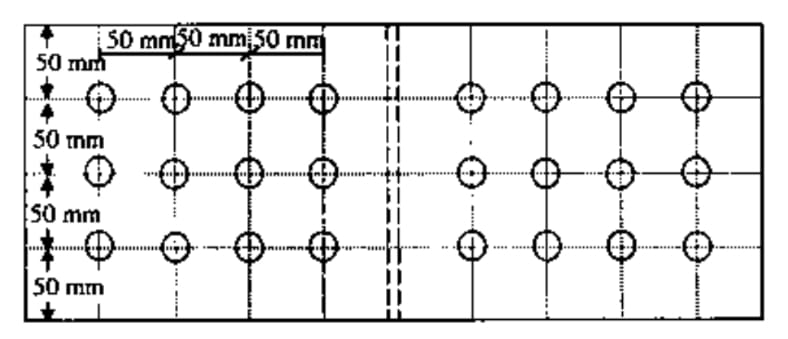
\includegraphics[scale=0.5]{figs/8332fb3c-532c-4d6c-a8c4-1f20c3321f4f.jpg} 
     \caption{}
     \label{fig:figure3}
 \end{figure}
\begin{enumerate}
\begin{multicols}{4}
\item 1083.6 kN 
\item 871.32 kN 
\item 541.8 kN 
\item 433.7 kN
\end{multicols}
\end{enumerate}
%------------------- Q33 -------------------%
\noindent\item Two plates, subjected to direct tension, each of 10 mm thickness and having widths of 100 mm and 175 mm, respectively are to be fillet welded with an overlap of 200 mm. Given that the permissible weld stress is 110 MPa and the permissible stress in steel is 150 MPa, the length of the weld required using the maximum permissible weld size as per IS:800-1984 is \hfill{\brak{\text{GATE CE 2010}}}

\begin{figure}[H]
     \centering
     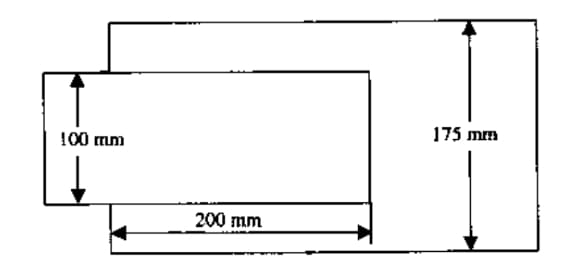
\includegraphics[scale=0.5]{figs/47c2880c-f6f6-44c0-8945-4aa142a40d60.jpg} 
     \caption{}
     \label{fig:figure4}
 \end{figure}
 \begin{enumerate}
\begin{multicols}{4}
\item 245.3 mm 
\item 229.2 mm 
\item 205.5 mm 
\item 194.8 mm
\end{multicols}
\end{enumerate}
%------------------- Q34 -------------------%
\noindent\item For the simply supported beam of length $L$, subjected to a uniformly distributed moment $M$ kN-m per unit length as shown in the figure, the bending moment (in kN-m) at the mid-span of the beam is
\hfill{\brak{\text{GATE CE 2010}}}

\begin{figure}[H]
     \centering
     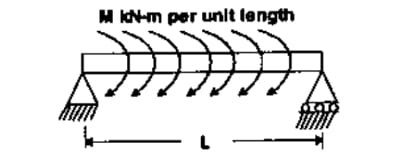
\includegraphics[scale=0.55]{figs/3d041fea-5713-4739-aa3e-a69aaeca9879.jpg} 
     \caption{}
     \label{fig:figure5}
 \end{figure}
 \begin{enumerate}
\begin{multicols}{4}
\item zero 
\item $M$ 
\item $ML$ 
\item $M/L$
\end{multicols}
\end{enumerate}
%------------------- Q35 -------------------%
\noindent\item A disc of radius $r$ has a hole of radius $\frac{r}{2}$ cut-out as shown. The centroid of the remaining disc (shaded portion) at a radial distance from the centre “O” is

\hfill{\brak{\text{GATE CE 2010}}}

\begin{figure}[H]
     \centering
     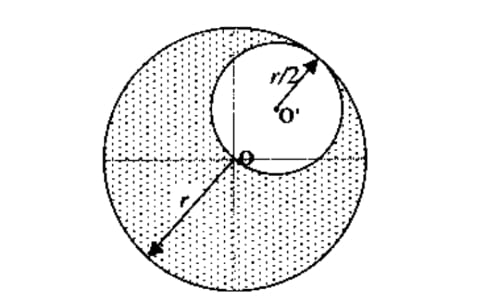
\includegraphics[scale=0.55]{figs/412a18c6-0377-40d3-8e64-77d6fc371075.jpg} 
     \caption{}
     \label{fig:figure6}
 \end{figure}
\begin{enumerate}
\begin{multicols}{4}
\item $\frac{r}{2}$ 
\item $\frac{r}{3}$ 
\item $\frac{r}{6}$ 
\item $\frac{r}{8}$
\end{multicols}
\end{enumerate}

%------------------- Q36 -------------------%
\noindent\item A three hinged parabolic arch having a span of 20 m and a rise of 5 m carries a point load of 10 kN at quarter span from the left end as shown in the figure. The resultant reaction at the left support and its inclination with the horizontal are respectively
\hfill{\brak{\text{GATE CE 2010}}}

\begin{figure}[H]
     \centering
     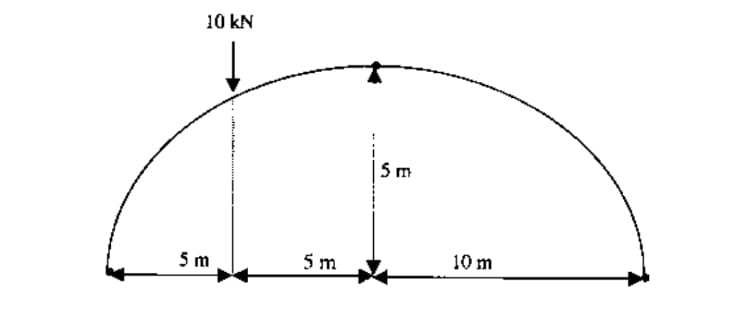
\includegraphics[scale=0.55]{figs/32b8c197-51f7-4381-b234-407edc801822.jpg} 
     \caption{}
     \label{fig:figure7}
 \end{figure}
\begin{enumerate}
\begin{multicols}{2}
\item 9.01 kN and $56.31^\circ$ 
\item 9.01 kN and $33.69^\circ$ 
\item 7.50 kN and $56.31^\circ$ 
\item 2.50 kN and $33.69^\circ$
\end{multicols}
\end{enumerate}
%------------------- Q37 -------------------%
\noindent\item The vertical stress at point $P_1$ due to the point load $Q$ on the ground surface as shown in figure is $\sigma_z$. According to Boussinesq's equation, the vertical stress at point $P_2$ shown in figure will be
\hfill{\brak{\text{GATE CE 2010}}}

\begin{figure}[H]
     \centering
     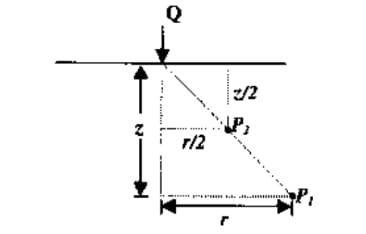
\includegraphics[scale=0.55]{figs/e4388fce-713b-4dc9-a1a5-4b431f7ae7ed.jpg} 
     \caption{}
     \label{fig:figure8}
 \end{figure}
\begin{enumerate}
\begin{multicols}{4}
\item $\frac{\sigma_z}{2}$ 
\item $\sigma_z$ 
\item $2\sigma_z$ 
\item $4\sigma_z$
\end{multicols}
\end{enumerate}
%------------------- Q38 -------------------%
\noindent\item An open ended steel barrel of 1 m height and 1 m diameter is filled with saturated fine sand having coefficient of permeability of $10^{-2}$ m/s. The barrel stands on a saturated bed of gravel. The time required for the water level in the barrel to drop by 0.75 m is \hfill{\brak{\text{GATE CE 2010}}}
\begin{enumerate}
\begin{multicols}{4}
\item 58.9 s 
\item 75 s 
\item 100 s 
\item 150 s
\end{multicols}
\end{enumerate}
%------------------- Q39 -------------------%
\noindent\item The ultimate load capacity of a 10 m long concrete pile of square cross section 500 mm $\times$ 500 mm driven into a homogeneous clay layer having undrained cohesion value of 40 kPa is 700 kN. If the cross section of the pile is reduced to 250 mm $\times$ 250 mm and the length of the pile is increased to 20 m, the ultimate load capacity will be
\hfill{\brak{\text{GATE CE 2010}}}
\begin{enumerate}
\begin{multicols}{4}
\item 350 kN 
\item 632.5 kN 
\item 722.5 kN 
\item 1400 kN
\end{multicols}
\end{enumerate}
\setlength{\parindent}{0pt}
\setlength{\parskip}{0.5cm}


%------------------- Q40 -------------------%
\noindent\item For a rectangular channel section, {Group-I} lists geometrical elements and {Group-II} gives proportions for hydraulically efficient section. 

\begin{table}[H]
\centering
\begin{tabular}{l l}
Group-I & Group-II  \\
P. Top width     & 1. $y_c/2$ \\
Q. Perimeter    & 2.  $y_c$     \\
R. Hydraulic Radius    & 3.  $2y_c$          \\
S. Hydraulic Depth    & 4. $y_c$
\end{tabular}
\label{table3}
\end{table}
$y_c$ is the flow depth corresponding to hydraulically efficient sections. The correct match of {Group-I} with {Group-II} is
\hfill{\brak{\text{GATE CE 2010}}}
\begin{enumerate}
\begin{multicols}{4}
\item P-2, Q-4, R-1, S-3 
\item  P-3, Q-1, R-4, S-2 
\item  P-3, Q-4, R-1, S-2 
\item  P-3, Q-4, R-2, S-1
\end{multicols}
\end{enumerate}
%------------------- Q41 -------------------%
\noindent\item The Froude number of flow in a rectangular channel is 0.8. If the depth of flow is 1.5 m, the critical depth is
\hfill{\brak{\text{GATE CE 2010}}}
\begin{enumerate}
\begin{multicols}{4}
\item 1.80 m 
\item 1.56 m 
\item 1.36 m 
\item 1.29 m
\end{multicols}
\end{enumerate}
%------------------- Q42 -------------------%
\noindent\item A well of diameter 20 cm fully penetrates a confined aquifer. After a long period of pumping at a rate of 2720 litres per minute, the observations of drawdown taken at 10 m and 100 m distances from the center of the well are found to be 3 m and 0.5 m respectively. The transmissivity of the aquifer is
\hfill{\brak{\text{GATE CE 2010}}}
\begin{enumerate}
\begin{multicols}{4}
\item 676 m$^2$/day 
\item 576 m$^2$/day 
\item 526 m$^2$/day 
\item 249 m$^2$/day
\end{multicols}
\end{enumerate}
%------------------- Q43 -------------------%
\noindent\item If the BOD$_5$ of a wastewater sample is 75 mg/L and reaction rate constant $k$ (base $e$) is 0.345 per day, the amount of BOD remaining in the given sample after 10 days is
\hfill{\brak{\text{GATE CE 2010}}}
\begin{enumerate}
\begin{multicols}{4}
\item 3.21 mg/L 
\item 3.45 mg/L 
\item 3.69 mg/L 
\item 3.92 mg/L
\end{multicols}
\end{enumerate}
%------------------- Q44 -------------------%
\noindent\item Consider the following statements in the context of geometric design of roads: \\begin{align*}0.1cm]
I: A simple parabolic curve is an acceptable shape for summit curves \\ 
II: Comfort to passengers is an important consideration in the design of summit curves \\begin{align*}0.2cm]
The correct option evaluating the above statements and their relationship is
\hfill{\brak{\text{GATE CE 2010}}}\newline
A.\ I is true, II is false \\
B.\ I is true, II is true, and II is the correct reason for I \\
C.\ I is true, II is true, and II is NOT the correct reason for I \\
D.\ I is false, II is true

%------------------- Q45 -------------------%
\noindent\item The design speed for a two-lane road is 80 kmph. When a design vehicle with a wheelbase of 6.6 m is negotiating a horizontal curve on that road, the off-tracking is measured as 0.096 m. The required widening of carriageway of the two-lane road on the curve is approximately
\\ \hfill{\brak{\text{GATE CE 2010}}}
\begin{enumerate}
\begin{multicols}{4}
\item 0.55 m 
\item 0.65 m 
\item 0.75 m 
\item 0.85 m
\end{multicols}
\end{enumerate}
%------------------- Q46 -------------------%
\noindent\item Consider the following statements in the context of cement concrete pavements: \\begin{align*}0.1cm]
I: Warping stresses in cement concrete pavements are caused by the seasonal variation in temperature \\ 
II: Tie bars are generally provided across transverse joints of cement concrete pavements \\begin{align*}0.2cm]
The correct option evaluating the above statements is
\hfill{\brak{\text{GATE CE 2010}}}
\begin{enumerate}
\begin{multicols}{4}
\item I: True, II: False 
\item I: False, II: True 
\item I: True, II: True 
\item I: False, II: False
\end{multicols}
\end{enumerate}
%47%
\noindent\item A bench mark has been established at the soffit of an ornamental arch at the known elevation of 100.0 m above mean sea level. The back sight used to establish height of instrument is an inverted staff reading of 2.105 m. A forward sight reading with normally held staff of 1.105 m is taken on a recently constructed plinth. The elevation of the plinth is

\setlength{\parskip}{0.5cm}

\hfill{\brak{\text{GATE CE 2010}}}
\begin{enumerate}
\begin{multicols}{4}
\item 103.210 m
\item 101.000 m
\item 99.000 m
\item 96.790 m
\end{multicols}
\end{enumerate}

\setlength{\parskip}{0.5cm}

\noindent{Common Data for Questions 48 and 49:}

\noindent Ion concentrations obtained for a groundwater sample (having pH = 8.1) are given below
\begin{table}[H]
\resizebox{\textwidth}{!}{%
\begin{tabular}{|c|c|c|c|c|c|c|}
\hline
Ion & Ca\(^{2+}\) & Mg\(^{2+}\) & Na\(^+\) & HCO\(_3^-\) & SO\(_4^{2-}\) & Cl\(^-\) \\
\hline
Ion concentration (mg/L) & 100 & 6 & 15 & 250 & 45 & 39 \\
\hline
Atomic Weight & Ca = 40 & Mg = 24 & Na = 23 & H = 1, C = 12, O = 16 & S = 32, O = 16 & Cl = 35.5 \\
\hline
\end{tabular}%
}
\label{table4}
\end{table}
%48%
\noindent\item Total hardness (mg/L as CaCO\(_3\)) present in the above water sample is

\setlength{\parskip}{0.5cm}

\hfill{\brak{\text{GATE CE 2010}}}
\begin{enumerate}
\begin{multicols}{4}
\item 205
\item 250
\item 275
\item 308
\end{multicols}
\end{enumerate}
\setlength{\parskip}{0.5cm}
%49%
\noindent\item Carbonate hardness (mg/L as CaCO\(_3\)) present in the above water sample is

\setlength{\parskip}{0.5cm}

\hfill{\brak{\text{GATE CE 2010}}}
\begin{enumerate}
\begin{multicols}{4}
\item 205
\item 250
\item 275
\item 289
\end{multicols}
\end{enumerate}

\setlength{\parskip}{0.5cm}

\noindent{Common Data for Questions 50 and 51:}

\noindent The moisture holding capacity of the soil in a 100 hectare farm is 18 cm/m. The field is to be irrigated when 50 percent of the available moisture in the root zone is depleted. The irrigation water is to be supplied by a pump working for 10 hours a day, and water application efficiency is 75 percent. Details of crops planned for cultivation are as follows

\begin{table}[H]
\centering
\begin{tabular}{|c|c|c|}
\hline
Crop & Root zone depth (m) & Peak rate of moisture use (mm/day) \\
\hline
X & 1.0 & 5.0 \\
Y & 0.8 & 4.0 \\
\hline
\end{tabular}
\label{table5}
\end{table}
%50%
\noindent\item The capacity of irrigation system required to irrigate crop 'X' in 36 hectares is

\setlength{\parskip}{0.5cm}

\hfill{\brak{\text{GATE CE 2010}}}
\begin{enumerate}
\begin{multicols}{4}
\item 83 litres/sec
\item 67 litres/sec
\item 57 litres/sec
\item 53 litres/sec
\end{multicols}
\end{enumerate}

\setlength{\parskip}{0.5cm}
%51%
\noindent\item The area of crop 'Y' that can be irrigated when the available capacity of irrigation system is 40 litres/sec is

\setlength{\parskip}{0.5cm}

\hfill{\brak{\text{GATE CE 2010}}}
\begin{enumerate}
\begin{multicols}{4}
\item 40 hectares
\item 36 hectares
\item 30 hectares
\item 27 hectares
\end{multicols}
\end{enumerate}

\noindent{Statement for Linked Answer Questions 52 and 53:}

A doubly reinforced rectangular concrete beam has a width of 300 mm and an effective depth of 500 mm. The beam is reinforced with 2200 mm\(^2\) of steel in tension and 628 mm\(^2\) of steel in compression. The effective cover for compression steel is 50 mm. Assume that both tension and compression steel yield. The grades of concrete and steel used are M20 and Fe250, respectively. The stress block parameters (rounded off to first two decimal places) for concrete shall be as per IS 456:2000.

\setlength{\parskip}{0.5cm}
%52%
\noindent\item The depth of neutral axis is

\setlength{\parskip}{0.5cm}

\hfill{\brak{\text{GATE CE 2010}}}
\begin{enumerate}
\begin{multicols}{4}
\item 205.30 mm
\item 184.56 mm
\item 160.91 mm
\item 145.30 mm
\end{multicols}
\end{enumerate}

\setlength{\parskip}{0.5cm}
%53%
\noindent\item The moment of resistance of the section is

\setlength{\parskip}{0.5cm}

\hfill{\brak{\text{GATE CE 2010}}}
\begin{enumerate}
\begin{multicols}{4}
\item 206.00 kN-m
\item 209.20 kN-m
\item 236.80 kN-m
\item 251.90 kN-m
\end{multicols}
\end{enumerate}

\setlength{\parskip}{0.5cm}

\noindent{Statement for Linked Answer Questions 54 and 55:}

The unconfined compressive strength of a saturated clay sample is 54 kPa.

\setlength{\parskip}{0.5cm}

\noindent\item The value of cohesion for the clay is

\setlength{\parskip}{0.5cm}

\hfill{\brak{\text{GATE CE 2010}}}
\begin{enumerate}
\begin{multicols}{4}
\item zero
\item 13.5 kPa
\item 27 kPa
\item 54 kPa
\end{multicols}
\end{enumerate}

\setlength{\parskip}{0.5cm}
\noindent\item If a square footing of size 4 m x 4 m is resting on the surface of a deposit of the above clay, the ultimate bearing capacity of the footing (as per Terzaghi’s equation) is

\setlength{\parskip}{0.5cm}

\hfill{\brak{\text{GATE CE 2010}}}
\begin{enumerate}
\begin{multicols}{4}
\item 1600 kPa
\item 316 kPa
\item 200 kPa
\item 100 kPa
\end{multicols}
\end{enumerate}

\section*{General Aptitude (GA) Questions}

\noindent{Q.56 -- Q.60 carry one mark each.}

\setlength{\parskip}{0.5cm}
%56%
\noindent \item \textit{Which of the following options is the closest in meaning to the word below:}\\


\hfill{\brak{\text{GATE CE 2010}}}
\begin{enumerate}
\begin{multicols}{4}
\item cyclic
\item indirect
\item confusing
\item crooked
\end{multicols}
\end{enumerate}

\setlength{\parskip}{0.5cm}
%57%
\noindent\item \textit{The question below consists of a pair of related words followed by four pairs of words. Select the pair that best expresses the relation in the original pair.}\\
Unemployed : Worker \hfill{\brak{\text{GATE CE 2010}}}
\begin{enumerate}
\begin{multicols}{2}
\item fallow : land
\item unaware : sleeper
\item wit : jester
\item renovated : house
\end{multicols}
\end{enumerate}

\setlength{\parskip}{0.5cm}
%58%
\noindent\item \textit{Choose the most appropriate word from the options given below to complete the following sentence:}
%59%
\noindent\textit{If we manage to \rule{2cm}{0.15mm} our natural resources, we would leave a better planet for our children.}

\hfill{\brak{\text{GATE CE 2010}}}
\begin{enumerate}
\begin{multicols}{4}
\item uphold
\item restrain
\item cherish
\item conserve
\end{multicols}
\end{enumerate}

\setlength{\parskip}{0.5cm}

\noindent\item \textit{Choose the most appropriate word from the options given below to complete the following sentence:}

\noindent\textit{His rather casual remarks on politics \rule{2cm}{0.15mm} his lack of seriousness about the subject.}

\hfill{\brak{\text{GATE CE 2010}}}
\begin{enumerate}
\begin{multicols}{4}
\item masked
\item belied
\item betrayed
\item suppressed
\end{multicols}
\end{enumerate}

\setlength{\parskip}{0.5cm}
%60%
\noindent\item 25 persons are in a room. 15 of them play hockey, 17 of them play football and 10 of them play both hockey and football. Then the number of persons playing neither hockey nor football is: \hfill{\brak{\text{GATE CE 2010}}}
\begin{enumerate}
\begin{multicols}{4}
\item 2
\item 17
\item 13
\item 3
\end{multicols}
\end{enumerate}

\setlength{\parskip}{0.5cm}

\noindent{Q.61 -- Q.65 carry two marks each.}

\setlength{\parskip}{0.5cm}

 \textit{Modern warfare has changed from large scale clashes of armies to suppression of civilian populations. Chemical agents that do their work silently appear to be suited to such warfare; and regretfully, there exist people in military establishments who think that chemical agents are useful tools for their cause.}

\vspace{0.3cm}
\noindent\item\textit{ Which of the following statements best sums up the meaning of the above passage:}

\hfill{\brak{\text{GATE CE 2010}}}

A.\ Modern warfare has resulted in civil strife. \\
B.\ Chemical agents are useful in modern warfare.\\
C.\ Use of chemical agents in warfare would be undesirable. \\
D.\ People in military establishments like to use chemical agents in war.

\noindent\item If 137 + 276 = 435, how much is 731 + 672?

\hfill{\brak{\text{GATE CE 2010}}}
\begin{enumerate}
\begin{multicols}{4}
\item 534
\item 1403
\item 1623
\item 1513
\end{multicols}
\end{enumerate}

\setlength{\parskip}{0.5cm}

\noindent\item 5 skilled workers can build a wall in 20 days; 8 semi-skilled workers can build a wall in 25 days; 10 unskilled workers can build a wall in 30 days. If a team has 2 skilled, 6 semi-skilled and 5 unskilled workers, how long will it take to build the wall?

\hfill{\brak{\text{GATE CE 2010}}}
\begin{enumerate}
\begin{multicols}{4}
\item 20 days
\item 18 days
\item 16 days
\item 15 days
\end{multicols}
\end{enumerate}

\setlength{\parskip}{0.5cm}

\noindent\item Given digits 2, 2, 3, 3, 3, 4, 4, 4, 4, how many distinct 4-digit numbers greater than 3000 can be formed?

\hfill{\brak{\text{GATE CE 2010}}}
\begin{enumerate}
\begin{multicols}{4}
\item 50
\item 51
\item 52
\item 54
\end{multicols}
\end{enumerate}

\noindent Hari (H), Gita (G), Irfan (I) and Saira (S) are siblings (i.e. brothers and sisters). All were born on 1\textsuperscript{st} January. The age difference between any two successive siblings (that is born one after another) is less than 3 years. Given the following facts:

\begin{itemize}
  \item[i.] Hari’s age + Gita’s age > Irfan’s age + Saira’s age.
  \item[ii.] The age difference between Gita and Saira is 1 year. However, Gita is not the oldest and Saira is not the youngest.
  \item[iii.] There are no twins.
\end{itemize}

\noindent \item  In what order were they born (oldest first)?

\hfill{\brak{\text{GATE CE 2010}}}
\begin{enumerate}
\begin{multicols}{2}
\item HSIG
\item SGHI
\item IGSH
\item IHSG
\end{multicols}
\end{enumerate}

\begin{center}
\section*{END OF QUESTION PAPER}
\end{center}

\end{enumerate}

\end{document}
	\item Verify that 
		\begin{align}
			\brak{\vec{A}-\vec{H}}^{\top}\brak{\vec{B}-\vec{C}} = 0
		\end{align}
  \input{solutions/1/3/5/Q_1.3.5.tex}
  \item Find the length of the altitude $AD_1$.
	  \\
		\solution 
		If the equation of $BC$ be $\vec{n}^\top\vec{x} =c$,
from
			\eqref{eq:geo-param},
\begin{align}
			\label{eq:app-geo-param-app}
	\vec{D}_1 = \vec{A} + k\vec{n}
	\\
	\implies AD_1 = \norm{\vec{D}_1 - \vec{A}}=\abs{k} \norm{\vec{n}}
			\label{eq:app-geo-param-app-PQ}
\end{align}
			From \eqref{eq:app-geo-param-app},
\begin{align}
	\vec{n}^{\top}  \vec{D}_1 = \vec{n}^{\top}  \vec{A} + k\norm{\vec{n}}^2
	\\
	\implies \abs{k} = 
	\frac{\abs{\vec{n}^{\top}\brak{\vec{D}_1 - \vec{A}}}}{\norm{\vec{n}}^2}
			\label{eq:app-geo-param-app-k}
			\\
	\implies AD_1 =\abs{k}  
		\norm{\vec{n}}	=
	\frac{\abs{\vec{n}^{\top}\vec{A} - c}}{\norm{\vec{n}}}
			\label{eq:app-PQ-final}
\end{align}
upon substituting from 
			\eqref{eq:app-geo-param-app-PQ}.
  \item Find $\vec{D}_1$.
	  \\
		\solution $\because \vec{D}_1$ lies on $BC$, 
\begin{align}
			\label{eq:app-BC-alt}
\vec{n}^\top\vec{D}_1 =c
\end{align}
and 
	$\because AD_1 \perp BC$,
\begin{align}
	\vec{m}^{\top}\brak{\vec{A}-\vec{D}_1} = 0
	\\
	\implies 
	\vec{m}^{\top}\vec{D}_1 = 
	\vec{m}^{\top}\vec{A}
			\label{eq:app-AD1-alt}
\end{align}
Clubbing
			\eqref{eq:app-BC-alt}
			and 
			\eqref{eq:app-AD1-alt},
\begin{align}
			\label{eq:app-D1-alt}
	\myvec{\vec{m} & \vec{n}}^\top\vec{D}_1 &= 
	   \myvec{
              \vec{m}^\top\vec{A}\\
	      c
	      }
\end{align}
\item 
All codes for this section are available at
\begin{lstlisting}
	codes/triangle/altitude.py
\end{lstlisting}
\end{enumerate}
